% mnras_template.tex
%
% LaTeX template for creating an MNRAS paper
%
% v3.0 released 14 May 2015
% (version numbers match those of mnras.cls)
%
% Copyright (C) Royal Astronomical Society 2015
% Authors:
% Keith T. Smith (Royal Astronomical Society)

% Change log
%
% v3.0 May 2015
%    Renamed to match the new package name
%    Version number matches mnras.cls
%    A few minor tweaks to wording
% v1.0 September 2013
%    Beta testing only - never publicly released
%    First version: a simple (ish) template for creating an MNRAS paper

%%%%%%%%%%%%%%%%%%%%%%%%%%%%%%%%%%%%%%%%%%%%%%%%%%
% Basic setup. Most papers should leave these options alone.
\documentclass[a4paper,fleqn,usenatbib]{mnras}

% MNRAS is set in Times font. If you don't have this installed (most LaTeX
% installations will be fine) or prefer the old Computer Modern fonts, comment
% out the following line
% \usepackage{newtxtext,newtxmath}
% Depending on your LaTeX fonts installation, you might get better results with one of these:
%\usepackage{mathptmx}
%\usepackage{txfonts}

% Use vector fonts, so it zooms properly in on-screen viewing software
% Don't change these lines unless you know what you are doing
\usepackage[T1]{fontenc}
\usepackage{ae,aecompl}

%%%%% AUTHORS - PLACE YOUR OWN PACKAGES HERE %%%%%

% Only include extra packages if you really need them. Common packages are:
\usepackage{graphicx}	% Including figure files
\usepackage{amsmath}	% Advanced maths commands
\usepackage{amssymb}	% Extra maths symbols
\usepackage{longtable}
\usepackage{pdflscape}
\usepackage{xspace}
\usepackage{verbatim}

% marconi section 7.1, 7.5
% tailo section 6.1

%%%%%%%%%%%%%%%%%%%%%%%%%%%%%%%%%%%%%%%%%%%%%%%%%%

%%%%% AUTHORS - PLACE YOUR OWN COMMANDS HERE %%%%%

% Please keep new commands to a minimum, and use \newcommand not \def to avoid
% overwriting existing commands. Example:
\newcommand{\ho}{$H_{0}$\xspace}
\newcommand{\ocen}{$\omega$~Cen\xspace}
%\newcommand{\vscomment}[1]{{\bf\textcolor{magenta}{#1}}
\providecommand{\vscomment}[1]{{\textcolor{magenta}{{VS: #1}}}\xspace}
%%%%%%%%%%%%%%%%%%%%%%%%%%%%%%%%%%%%%%%%%%%%%%%%%%

%%%%%%%%%%%%%%%%%%% TITLE PAGE %%%%%%%%%%%%%%%%%%%

% Title of the paper, and the short title which is used in the headers.
% Keep the title short and informative.
\title[Mid-IR RRL PLZ Relations in $\omega$ Cen]{The Carnegie RR Lyrae Program: The (Near- and??) Mid-Infrared RR Lyrae Period-Luminosity-Metallicity Relations in $\omega$~Cen}

% The list of authors, and the short list which is used in the headers.
% If you need two or more lines of authors, add an extra line using \newauthor
\author[M.~J.~Durbin et al.]{Meredith~J.~Durbin$^{1}$
Victoria Scowcroft$^{2}$
Wendy L. Freedman$^{3}$
Barry F. Madore$^{2}$
\newauthor Rachael L. Beaton$^{2}$
%Gurtina Besla$^{5}$ 
%Giuseppe Bono$^{6, 7}$
%Vittorio Braga$^{6, 7}$
%\newauthor Maria-Rosa Cioni$^{8, 9, 10}$
%Gisella Clementini$^{11}$
%Kathryn Johnston$^{12}$
%Nitya Kallivayalil$^{13}$
%\newauthor Juna Kollmeier$^{3}$
%David Law$^{1}$
%Steve Majewski$^{13}$
%Roeland van der Marel$^{1}$
%\newauthor Massimo Marengo$^{14}$
Andrew~J.~Monson$^{4}$
%Jill Neeley$^{14}$
%David Nidever$^{16}$ 
%\newauthor Grzegorz Pietrzynski$^{17, 18}$
Jeffrey Rich Jr.$^{2}$
Mark Seibert$^{2}$
%Horace Smith$^{19}$
%\newauthor Igor Soszynski$^{17}$
%Andrzej Udalski$^{17}$
\\
% List of institutions
$^1$ Space Telescope Science Institute, 3700 San Martin Drive, Baltimore, MD 21218, USA \\
$^2$ Observatories of the Carnegie Institution of Washington, 813 Santa Barbara St., Pasadena, CA 91101, USA \\
$^3$ Department of Astronomy and Astrophysics, University of Chicago, 5640 S Ellis Ave, Chicago, IL 60637, USA \\
%$^5$ Department of Astronomy and Steward Observatory, University of Arizona, 933 North Cherry Avenue,   Tucson, AZ 85721, USA \\
%$^6$ Univ. Roma ``Tor Vergata", Via della Ricerca Scientifica, 1 - 00133, Roma, Italy \\
%$^7$ INAF-OAR, via Frascati 33 - 00040, Monte Porzio Catone (RM), Italy \\
%$^8$ Universtat Potsdam, Institut fur Physik und Astronomie, Karl-Liebknecht-Str. 24/25, 14476 Potsdam, Germany \\
%$^9$ Leibniz-Institut fur Astrophysik Potsdam, An der Sternwarte 16, 14482 Potsdam, Germany \\
%$^{10}$ University of Hertfordshire, Physics, Astronomy and Mathematics, College Lane, Hatfield AL10 9AB, United Kingdom \\
%$^{11}$ INAF - Osservatorio Astronomico, Via Ranzani n. 1, 40127 Bologna, Italy \\
%$^{12}$ Department of Astronomy, Columbia University, New York, NY 10027, USA  \\
%$^{13}$ Department of Astronomy, University of Virginia, Charlottesville, VA 22904-0818, USA \\
%$^{14}$ Department of Physics and Astronomy, Iowa State University, Ames, IA, USA \\
$^{4}$ Department of Astronomy and Astrophysics, The Pennsylvania State University, 525 Davey Lab, University Park, PA, 16802, USA \\
%$^{16}$ Department of Astronomy, University of Michigan, Ann Arbor, MI 48109, USA \\
%$^{17}$ Warsaw University Observatory Al. Ujazdowskie 4, 00-478 Warszawa, Poland \\
%$^{18}$ Departamento de Astronomia, Universidad de Concepcion, Casilla 160-C, Chile \\
%$^{19}$ Department of Physics and Astronomy, Michigan State University, East Lansing, MI, USA 48824 \\
}

% These dates will be filled out by the publisher
\date{Accepted XXX. Received YYY; in original form ZZZ}

% Enter the current year, for the copyright statements etc.
\pubyear{2016}

% Don't change these lines
\begin{document}
\label{firstpage}
\pagerange{\pageref{firstpage}-\pageref{lastpage}}
\maketitle

% Abstract of the paper
\begin{abstract}
\end{abstract}

% Select between one and six entries from the list of approved keywords.
% Don't make up new ones.
\begin{keywords}
keyword1 - keyword2 - keyword3
\end{keywords}

%%%%%%%%%%%%%%%%%%%%%%%%%%%%%%%%%%%%%%%%%%%%%%%%%%

%%%%%%%%%%%%%%%%% BODY OF PAPER %%%%%%%%%%%%%%%%%%

%% IMPORTANT NOTES FROM VS:

% MNRAS is a UK journal - change your spellcheck language in your editor to British English. 
% Correct plural of RR Lyrae is RR Lyrae variables (technically, singular should be RR Lyrae variable, as RR Lyrae itself is a named object)
% Use 1 dash - for a minus sign in math mode
% Use 2 dashes -- to hyphenate words
% Use 3 dashes --- to put a dash between parts of a sentence or to denote a minus sign outside of math mode

% ^^^ From the MNRAS style guide:

% Hyphens (one dash in LaTeX) should be used for compound adjectives (e.g. low-density gas, least-squares fit, two-component model). This also applies to simple adjectival units (e.g. 1.5-m telescope, 284.5-nm line), but not to complex units or ranges, which could become cumbersome (e.g. 15 km sÐ1 feature, 100Ð200 µm observations). Some words (e.g. time-scale) are always hyphenated as part of journal style (see below). 

% N-rules (two dashes in LaTeX): these are longer than hyphens and are used (i) to separate key words, (ii) as parentheses (e.g. the results Ð assuming no temperature gradient Ð are indicative of É), (iii) to denote a range (e.g. 1.6Ð2.2 µm), and (iv) to denote the joining of two words (e.g. KolmogorovÐSmirnov test, HerbigÐHaro object). 

% M-rules (three dashes in TeX/LaTeX) are not used in MNRAS.

% Figures and tables can go at their appropriate places in the document rather than at the end. 
% To update bibtex source run ads_importer.py omegaCen_mnras_2015 after latex, then run latex, bibtex, latex, latex (ads_importer.py is available from VS's github, rely's on ADS style refs).

\section{Introduction}
\label{sec:intro}

%Suggested intro structure from RLB:
%
%\begin{enumerate}
%	\item $H_{0}$ and the need for other distance ladders. $\checkmark$
%	\item RR Lyrae as a good local standard candle, particularly in the mid-IR $\checkmark$
%	\item MidIR RRL as a standard candle that needs auxiliary analysis in order to be applied
%	\item The need to constrain metallicity effects, using the well known horizontal branch dependencies on metallicity as a basis
%	\item One such analysis $\rightarrow$ empirical study of metallicity term in the NIR/MIR - literature not settled.
%	\item Murareva et al. (2015), table 3 for NIR
%	\item This work (Durbin et al. 2016) explores the MIR metallicity effect {\bf which has not previously been explored empirically}
%	\item Establish $\omega$ Cen as the best place to do this test
%	\item Be clear that prior analyses of $\omega$ Cen have been inconclusive in optical compared to theoretical expectations
%	\item Outline of paper.
%\end{enumerate}
%
%{\bf Remember to go from BIG PICTURE to FINE DETAIL. Go from the WHY to the HOW.}

% MARK'S IDEAS
% the introduction isn't specific enough to the paper at hand
% p1: desc of omega cen - minor history, distance, radius, weirdness, etc - unusual glob clust. that's what makes it natural lab for studying eff of metallicity on distance indicators
% p2: summary of what we know about metallicity of omega cen - nir, mir
% p3: use this to investigate effect on rrl PL relation
% p4: [fe/h] on rrl in nir, mir
% p5: use rrl as first step in dist ladder, alt to cepheids to get to h0 with population ii only, crrp/chp
% p6: paper outline

% put propid in data section
% no mention of cepheids
% don't talk about standard candle criteria
% cite madore 2013 when talking about dispersion
% we don't know if metallicity is most important factor in driving dispersion-has yet to be demonstrated to any significant level

Given its proximity, size, and complexity, $\omega$~Centauri (NGC 5139) has become one of the most well-studied Galactic globular clusters (GGCs) \citep{
    2002ASPC..265.....V}. It has a mass of approximately $4 \times 10^6~M_{\odot}$ \citep{2013MNRAS.429.1887D}, and a tidal radius of 88~pc \citep{2005MNRAS.360..631M}. $\omega$~Cen's close proximity to Earth \citep[$d \sim 5.5$~kpc, e.g.][]{2006ApJ...652..362D, 2001AJ....121.3089T} allows us to resolve the stellar population of this dense cluster. 

Although it has been subject to decades of investigations, the true nature of $\omega$~Cen remains unclear. It is one of the most massive GGCs orbiting the Milky Way. It is significantly flattened \citep[$\epsilon = 1 - b/a = 0.17$][]{2005MNRAS.360..631M} and it does not show the levels of mass segregation in its stellar population that would be expected were it in equipartition \citep{2002ASPC..265...87A}. Additionally, \ocen was the first GGC discovered to comprise more than one stellar population \citep{1999Natur.402...55L}, breaking down the prevailing interpretation that GGCs were simple stellar populations with a single episode of star formation, hence a monolithic age and metallicity distribution.

There are at least seven distinct stellar populations in \ocen \citep{2016MNRAS.457.4525T}, with a spread in metallicity as large as $0.8$ to $1.4$~dex \citep{2014ApJ...791..107V, 2012ApJ...746...14M, 2010ApJ...722.1373J}. As all the stars in \ocen are at approximately the same distance from Earth\footnote{In this case, the spread in distance due to the depth of the cluster is negligible.}, it is the ideal testbed for studying the effects of changing metallicity on a population.

In this work we focus on the effects of changing metallicity on the RR Lyrae variables (RRL), specifically examining whether the period--luminosity (PL) relations in the near-- and mid--infrared (IR) are affected, and the magnitude of any such effects. $\omega$~Cen has been used previously for such studies, ranging from empirical tests in the optical \citep[e.g.][]{2003MNRAS.345...86O, 1991ApJ...373L..43L} and near--IR \citep[e.g.][]{2006MmSAI..77..245C, 2006ApJ...652..362D}, to semi--empirical tests using population synthesis techniques \citep{2016MNRAS.457.4525T}. 

This work is part of the Carnegie RR Lyrae Program (CRRP), a Warm {\it Spitzer} Exploration Science program with the aim of provide an independent, Population II anchor to the extragalactic distance scale. Tied to RR Lyrae variables with high--precision, geometric distances in the Milky Way, the CRRP will ultimately provide a single instrument measurement of $H_{0}$, independent of Cepheid measurements, putting important constraints on the external accuracy of the standard candle distance ladder, and the internal consistency of the distance measurements of Cepheids and RR Lyrae variables.
 
 Although observing RRL at mid--IR wavelengths dramatically reduces the effects of reddening and extinction \citep[$A_{[3.6]} \sim A_V / 16$][]{2005ApJ...619..931I}, a consensus has not been reached on the consequences of this shift to longer wavelengths on the metallicity term in the empirical RRL PL relation. Both theory and observation have demonstrated that the position of the horizontal branch in the optical colour--magnitude diagram is dependent on metallicity \citep[e.g.][]{2015ApJ...808...50M, 2004ApJS..154..633C, 2003MNRAS.344.1097B, 1994AJ....108..222N}. However, the size of the metallicity contribution in the infrared PL relation is yet to be settled in the literature, either from a theoretical or empirical standpoint. 
 
The most in--depth study of the effect of metallicity on the mid--IR PL relation to date comes from \citet{2014MNRAS.439.3765D}, who used WISE data \citep{2010AJ....140.1868W, 2013wise.rept....1C} to examine possible changes in the RRL PL relation in globular clusters with different metallicities. They found a moderate metallicity dependence of the [W1]\footnote{approximately equivalent to {\it Spitzer} $3.6~\mu$m band} PL relation, with $\gamma_{W1} = 0.106 \pm 0.023$~mag~dex$^{-1}$, slightly larger than their value for the near--IR, and approximately half that of the optical dependence \citep[$\gamma_{K} = 0.088 \pm 0.026$~mag~dex$^{-1}$, $\gamma_{V} = 0.232 \pm 0.020$~mag~dex$^{-1}$,][]{2013MNRAS.435.3206D}. The observational work of \citet{2015ApJ...807..127M} appears to confirm this result, favouring a low value of $\gamma_K$ for Milky Way and Large Magellanic Cloud RRL. However, the empirical study of \citet{2015AJ....150...90K} considers near--IR observations of RRL in the Carina dwarf Spheroidal (dSph) galaxy, this time testing different PL relations with a range of metallicity coefficients. Their results favour a larger value for $\gamma_K$ than \citet{2015PKAS...30..183D}, with average values of $\gamma_K \approx 0.18$~mag~dex$^{-1}$. This is consistent with the theoretical models by \citet{2015ApJ...808...50M}, who find that the metallicity dependence of the infrared PL relation is just as large as at optical wavelengths.

Our study is unique as it is the first study to use $\omega$~Cen to empirically measure the metallicity effect on the mid--IR RRL PL relation using metallicities of individual stars, rather than comparing the populations of RRL in different GGCs or dSph. Our approach --- studying only {\it differential photometric effects} --- removes the systematic uncertainties introduced by comparing populations at different distances with different levels of foreground extinction, and in some cases observed with different instruments.

The paper is set out as follows: Section~\ref{sec:observations} details the observations and data reduction. Section~\ref{sec:results} presents the photometry of the $\omega$~Cen RRL. Section~\ref{sec:pl_relation} describes the mid-IR PL relations and Section~\ref{sec:distance_moduli} discusses the application of these to a distance measurement of  $\omega$~Cen. Section~\ref{sec:metallicity} examines the effects of metallicity on RRL magnitudes and distance estimates. Section~\ref{sec:discussion} discusses the implications of this, and other systematic effects we consider in this work. In Section~\ref{sec:conclusions} we present our conclusions.




%In the era of `precision cosmology' it is important to fully understand all sources of uncertainty in our experiments. Although the results distance ladder measurements such as \citet{2011ApJ...730..119R} and \citet{2012ApJ...758...24F} agree very well, 
%%at $74.4\pm 2.5$~km~s$^{-1}$~Mpc$^{-1}$ and $74.3\pm2.6$~km~s$^{-1}$~Mpc$^{-1}$, respectively, 
%when we consider the latest results from {\it Planck} 
%%who find $67.48\pm0.98$~km~s$^{-1}$~Mpc$^{-1}$ \citep{2015arXiv150201589P},
% there is tension. The {\it Planck} study derives its measurement from a model of the cosmic microwave background (CMB), so is completely independent of the \citeauthor{2011ApJ...730..119R} and \citeauthor{2012ApJ...758...24F} results. Works such as \citet{2015ApJ...802...20R} and \citet{2014MNRAS.440.1138E} have examined the contribution of systematic uncertainties at the far end of the distance ladder to this tension. The CRRP is quantifying the systematic uncertainty in the standard candle distance ladder by making meaningful comparisons at the base of the Cepheid and RR Lyrae distance ladders in the mid--infrared, where distance measurements of similar precision are achievable. 

% A good local standard candle \citep[as defined by][]{1986ApJ...303....1A} has the following  features: a)~a physical basis, b)~objective measurable, c)~minimal corrections, and d)~small scatter. RR Lyrae variables (hereafter RRL) are excellent standard candles in the mid--infrared. As \citet{1986MNRAS.220..279L} demonstrated, unlike at optical wavelengths where their absolute magnitudes depend only on metallicity, in the infrared RRL follow a clear period--luminosity (PL) relation. The PL relation has a physical basis (i.e. the PL relation is directly linked to the period--radius relation), and both the period and luminosity of the RRL can be objectively measured. In the mid--IR minimal extinction corrections are required \citep[$A_{[3.6]} \approx A_{V}/16$,][]{2005ApJ...619..931I}, and the dispersion of the relation in the infrared has been shown to be small compared to optical wavelengths \citep{2015ApJ...808...50M, 2004ApJS..154..633C}. Through this decrease in dispersion we have found that the intrinsic width of the mid-IR PL for RRL is in fact \emph{smaller} than for Cepheids -- less than 0.05~mag compared to 0.10~mag \citep{2015ApJ...808...11N, 2011ApJ...743...76S}. This translates to a distance uncertainty for an individual RRL of below 2\% for RRL, compared to 4\% for Cepheids, at 3.6~$\mu$m. Thus, for nearby systems RRL are the most precise standard candles.



%RR Lyrae variables (hereafter RRL) are intrinsically fainter than Cepheids, and in the optical follow a much shallower, even horizontal, PL relation \citep{2004ApJS..154..633C}. Determining an accurate distance to an RRL in the $V$ band requires knowledge of its metallicity. However, \citet{1986MNRAS.220..279L} showed that the true power of RRL as distance indicators lies in the IR passbands. Recently, several groups have been studying the populations of RRL in globular clusters and nearby dwarf spheroidal galaxies in the infrared \citep[e.g.][and references therein]{2013ApJ...767...62G, 2014ApJ...786..147O, 2015ApJ...806..200C, 2015A&A...578A.128K}. Several Galactic RRL now have high precision geometric distances measured as part of the HST-Fine Guidance Sensor (HST-FGS) parallax program \citep{2011AJ....142..187B}, and can therefore be used to calibrate the absolute zero-point of the RRL PL relation.% and \textit{HST} parallaxes were obtained for several Galactic RRL calibrators \citep{2011AJ....142..187B}, where calibrators are RRL whose distances can be determined by both parallax and period-luminosity fitting. {\bf (Is that right? Should I be more general and say any object whose distance can be determined by more than one distance ladder method?)}

%Distance measurements made in the mid-IR benefit from reduced extinction effects, where $A_{[3.6]}$ and $A_{[4.5]}$ are 16 to 20 times lower than $A_V$ \citep{1989ApJ...345..245C, 2005ApJ...619..931I}. Additionally, the precision of distances obtained from the RRL PL relation is increased. At the wavelengths observed by Warm \textit{Spitzer} (3.6 and 4.5~$\mu$m) we do not see photospheric effects, but only the effects of temperature driving the pulsation; essentially, the mid-infrared light curve is tracing the change in radius of the star through the pulsation cycle. A by-product of this effect is that the intrinsic width of the RRL PL relation is also minimised in the mid-IR. The PL relation for pulsational variables can be thought of as a two-dimensional projection of the three-dimensional period-luminosity-colour relation (see figure 3 of \citet{1991PASP..103..933M} for a graphical representation). As the effects of temperature are reduced, the colour-width of the PL decreases in the mid-IR. As one moves from the optical to the mid-IR, the slope of the PL relation steepens and its dispersion dramatically decreases; the slope should asymptotically approach the predicted slope of the period-radius relation, resulting in a slope between $-2.4$ and $-2.8$, confirmed empirically by \citet{2013ApJ...776..135M}. Through this decrease in dispersion we have found that the intrinsic width of the mid-IR PL for RRL is in fact \emph{smaller} than for Cepheids -- less than 0.05~mag compared to 0.10~mag \citep{2015ApJ...808...11N}. This translates to an uncertainty on an individual RRL of below 2\%, compared to 4\% for Cepheids. Thus, for nearby systems RRL are the most precise standard candles.
%
%In this work we focus on the effects of metallicity on the RRL PL relation in the mid-infrared. Several Galactic Globular Clusters are being observed as part of CRRP, but $\omega$~Cen is unique in that it exhibits a measurable spread in metallicity \citep{1975ApJ...201L..71F, 2007ApJ...663..296V, 2014ApJ...791..107V}.
%
%There are very few metallic or molecular transition lines in the mid-IR at typical RRL temperatures, so the effects of metallicity on luminosity should be minimised. However, $\omega$~Cen provides the ideal environment for a direct empirical test. Such an effect is not out of the realm of possibility; for example, the strength of the CO band head at 4.5~$\mu$m has been found to have a significant effect on Cepheid colours \citep{2010ApJ...709..120M}, and has such prevented the IRAC 4.5~$\mu$m Cepheid observations from being used for distance measurements in the CHP \citep{2011ApJ...743...76S, 2012ApJ...759..146M, 2016ApJ...816...49S}. Our concern in this program is systematic precision, and therefore we must test for any potential effects directly.
%
\section{Observations \& Data Reduction}
\label{sec:observations}
This work combines mid-IR observations from the CRRP Warm {\it Spitzer} program with supporting near-IR observations from the FourStar instrument \citep{2013PASP..125..654P} on the Baade-Magellan telescope at Las Campanas Observatory. Figure~\ref{fig:omegaCen_fields} shows a $K_s$-band FourStar image with the {\it Spitzer} fields outlined, and the positions of known RRL from \citet{2004A&A...424.1101K} indicated by circles (fundamental mode, RRab) or triangles (first overtone, RRc). 

\begin{figure*}
\begin{center}
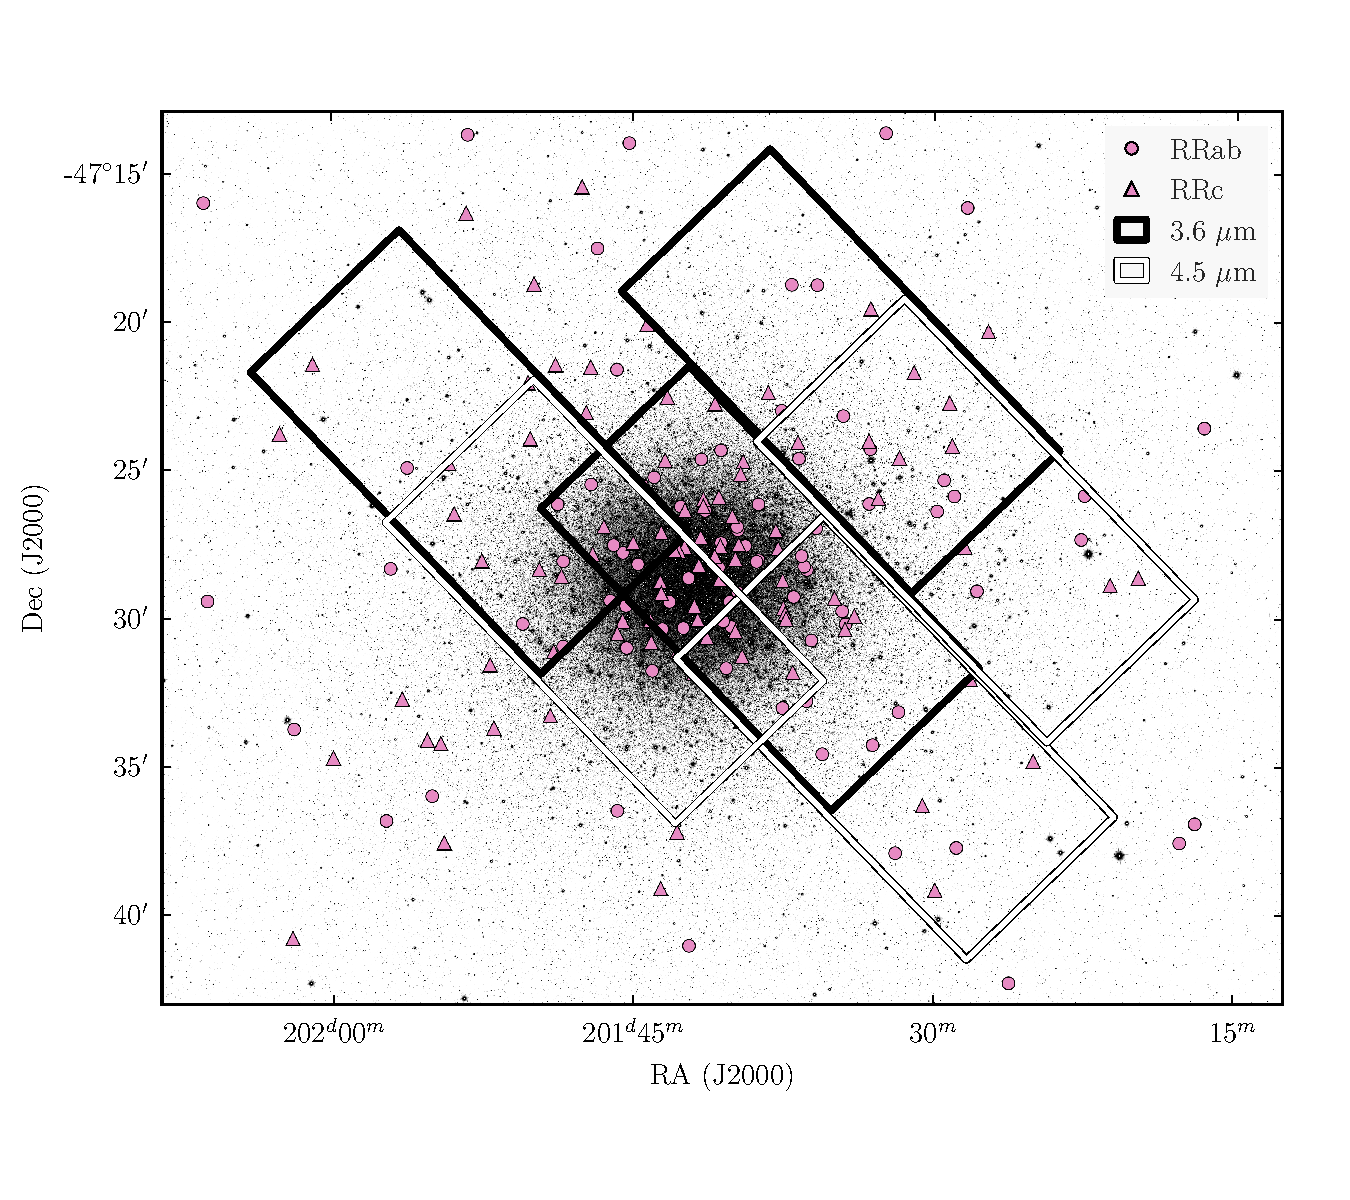
\includegraphics[width=160mm, trim=1cm 0 1cm 0]{reworked_fitting_code/final_plots/omegacen_coverage_map_new.pdf}
\caption{A $K_s$-band image of $\omega$~Cen from the FourStar camera, overlaid with a catalog of RRL from \citet{2004A&A...424.1101K} and footprints of the {\it Spitzer} IRAC fields. The circular points are RRab's and the triangular points are RRc's; we adopt this convention throughout the paper. The three black rectangle outlines are the IRAC field of view for each pointing in the 3.6~$\mu$m channel, and the white rectangle outlines show the same for 4.5~$\mu$m.} 
\label{fig:omegaCen_fields}
\end{center}
\end{figure*}

\subsection{{\em Spitzer} Data}
\label{sec:spitzer_reduction}
The \textit{Spitzer} observations for this work were taken as part of the CRRP \citet[][{\it Spitzer} PID 90002]{2012sptz.prop90002F}. Three fields in $\omega$~Cen were chosen; their positions are shown in Figure~\ref{fig:omegaCen_fields}. To obtain optimal RRL light curves we observed each field 12 times over approximately 16 hours (0.67~days), roughly corresponding to the longest period RRL we expected in the field and ensuring full phase coverage of all RRL. The observations of all three fields were taken on 2013 May 10 and 2013 May 11. Each field was observed using the {\it Spitzer} InfraRed Array Camera (IRAC) \citep{2004ApJS..154...10F} with a 30~s frame time with a medium scale, gaussian 5-point dither pattern to mitigate any image artefacts. Images were collected in both the 3.6 and 4.5~$\mu$m channels. 
The elongated field shapes come from the design of IRAC; while the [3.6] channel is collecting on-target data, the [4.5] channel collects off target data ``for free'', and vice versa. We chose to include these off-target fields to maximise the number of RRL in our final sample and to increase the legacy value of our data set to the community. 

The science images were created using \textsc{mopex} \citep{2006SPIE.6274E..0CM}, first running overlap correction on the corrected basic calibrated data frames (cBCDs) then mosaicking the original, under--sampled 1.2 arcsec scale images to a resolution of 0.6 arcsec pixel scale using the drizzle algorithm. Mosaicked location-correction images were created at the same time. The science mosaics have a signal to noise of approximately 100 at the brightness level of the RRL in both bands. 

% say resolution/FWHM
PSF photometry was performed on the mosaicked images using {\sc daophot} and {\sc allframe} \citep{1987PASP...99..191S, 1994PASP..106..250S}. The PSF model was created for each field/filter combination using the first epoch data and was applied to every epoch. As the observations were taken temporally close together the effects of telescope rotation between epochs on the mosaicked PSF were minimal, so making a single good PSF model for each field/filter combination proved to be more efficient and just as accurate as creating one for every epoch. 

Master star lists for {\sc allframe} were created for each filter/field combination using a median mosaicked image created by {\sc mopex}. We did not use the same single master star list for both filters as only a small proportion ($1/3$) of the [3.6] and [4.5] fields overlap each other. Instead we performed separate {\sc allframe} reductions for each filter, and combined the results after the fact using {\sc daomatch} and {\sc daomaster}. Our mid-IR photometry is calibrated to the standard system set by \citet{2005PASP..117..978R}.

%% 0.159 arcsec/pixel scale of the $K_s$ band image compared to the 0.6 arcsec/pixel scale

\subsection{FourStar Data}
\label{sec:fourstar_reduction}

% compare FWHMs not pixel scale
$J$, $H$ and $K_s$ data were taken with the FourStar instrument on the Baade-Magellan telescope at Las Campanas Observatory \citep{2013PASP..125..654P} on the nights of 2013 June 25, 2013 June 27, and 2013 June 28. Four epochs were obtained each night in each filter for a total of 12 epochs, with a typical image quality of $\text{FWHM} =0.6$ arc-seconds in the $K_{S}$ band. A mosaic of $5\times3$ slightly overlapping pointings (tiles), each with FourStar's native $10.9 \times 10.9$ arc-minute field of view, covered a $50\times30$ arc-minute field of view centred on $\omega$~Cen. Each tile consists of a 5 point dither pattern with a 5.8 second exposure time. Stacked mosaics of the entire field were made as well as individual tiles using a customised pipeline for FourStar data. The purpose of the individual tiles is to provide photometry with better time resolution than the large mosaic. 

PSF photometry of the tiles was performed using \textsc{daophot} and \textsc{allframe} \citep{1987PASP...99..191S, 1994PASP..106..250S}. A PSF model was created for each epoch/tile/filter combination. A master star list for \textsc{allframe} was created from the final $K_s$ mosaic and the multi-wavelength/epoch results were combined using \textsc{daomatch} and \textsc{daomaster}. Our final photometry is calibrated to the 2MASS standard system \citep{2006AJ....131.1163S}. 

\subsection{Crowding}
\label{sec:crowding}

\vscomment{Expand this section to include the crowded/uncrowded image cutouts.}

The primary limiting factor in the photometric precision is crowding. To assess crowding for individual RRLs, we compared the {\it Spitzer} images to the higher resolution FourStar $K_s$-band image. The 0.159 arcsec/pixel scale of the $K_s$-band image compared to the 0.6 arcsec/pixel scale of the IRAC images enabled us to more accurately determine which stars were significantly contaminated. RRL were determined to be contaminated if there were one or more resolved stars in the $K_s$-band image within a 3.6 arc-second (6 resampled IRAC pixels) radius of the RRL. 77 RRLs out of the original \citet{2004A&A...424.1101K} catalog of 192 were rejected due to crowding. Another 13 were outside the FourStar mosaic field of view, and four more were found to be unusable due to other image artefacts.

\section{Results}
\label{sec:results}

Our final photometry catalog, including magnitudes and uncertainties for $J\!H\!K_s$, [3.6], and [4.5], is presented in Table~\ref{tab:everything}. The average magnitudes presented in Table~\ref{tab:everything} are flux averages, and the photometric uncertainties of the time series data are the error on the mean. 
{\bf Note: this will not be an appendix in the final draft, we're just putting it there for now because it's huge.}

Our full, uncrowded RRL sample consists of 96 stars in $J$ and $H$, 98 in $K_s$, 38 in [3.6], and 42 in [4.5]; the small number of RRL in the IRAC bands compared to the FourStar bands is due to the smaller coverage of the IRAC pointings (see Figure~\ref{fig:omegaCen_fields}) and crowding effects due to IRAC's lower resolution. For the PL fitting, detailed in Section~\ref{sec:pl_relation}, we use only the stars for which we have photometry in all five bandpasses, ensuring that the same range of periods and metallicities are sampled for each wavelength. This helps to reduce any biases that may be introduced by non--uniform sampling in the distance moduli fits in Section~\ref{sec:distance_moduli}. Our final RRL sample consists of 24 stars, with 12 each of RRab's and RRc's.

\section{Period-Luminosity Relations}
\label{sec:pl_relation}

We fit PL relations using the theoretical near-infrared PL relation parameters presented in \citet{2015ApJ...808...50M} for the $JHK_s$ bands, and the empirical PL relation parameters derived from photometry of RRLs in the globular cluster M4 (NGC 6121) from \citet{2015ApJ...808...11N} for the IRAC bands. With the use of preexisting PL relation coefficients, the distance modulus becomes the only free parameter in our fit. We fit all distance moduli using an unweighted least-squares method, and fit the distance modulus to each pulsation mode in each wavelength separately. We also refine the fit by sigma-clipping the residuals of the [3.6] fit at a $2\sigma$ level, resulting in the rejection of two more stars.

For the mid-IR we use the PL relations from \citet{2015ApJ...808...11N}, as described in Table~\ref{tab:pl_table_m4}. These relations take the form
\begin{equation}
\label{eqn:neeley_pl}
M = a + b \times (\log (P) -  \log(P_0))
\end{equation}
where $a$ and $b$ are empirically derived coefficients and $P_0$ is the absolute value of the logarithm of the mean period of the M4 RRL sample. We calculate the absolute PL zero-points, $a$, by adopting \citeauthor{2015ApJ...808...11N}'s M4 distance modulus of $\mu=11.399$ mag.


\begin{table}
\centering
%% Adding the { } around the equation in the caption prevents it putting a line break in the middle of it
\caption{Empirical mid-IR RRL period-luminosity relation coefficients \citep{2015ApJ...808...11N}, for relations of the form ${M = a + b \times (\log (P) - \log(P_0))}$ (Eqn.~\ref{eqn:neeley_pl}) with observed dispersion $\sigma$. These relations are derived from RRL in the globular cluster M4.} 
\label{tab:pl_table_m4}
\begin{tabular}{l||c|c|c|c|c|r} 
\hline \hline
Band & Mode & $a$ & $b$ & $\log P_0$ & $\sigma$ \\
\hline
$[3.6]$ & RRab & $-0.558$ & $-2.370$ & $-0.260$ & $0.040$ \\
            & RRc & $-0.192$ & $-2.658$ & $-0.550$ & $0.079$ \\
$[4.5]$ & RRab & $-0.593$ & $-2.355$ & $-0.260$ & $0.045$ \\
            & RRc & $-0.240$ & $-2.979$ & $-0.550$ & $0.057$ \\ 
            \hline
\end{tabular}
\end{table}

The $JHK_s$ RRL PL relations are described in Table~\ref{tab:pl_table_theo}. The relations take the form
\begin{equation}
\label{eqn:marconi_pl}
M = a + b\times\log P + c\times[\text{Fe/H}]
\end{equation}
where $a$, $b$, and $c$ are theoretically derived coefficients.

\begin{table}
\centering
\caption{Theoretical near-IR RRL period-luminosity relation coefficients \citep{2015ApJ...808...50M}, for relations of the form ${M = a + b \times \log P + c \times [\text{Fe/H}]}$ (Eqn.~\ref{eqn:marconi_pl}) with modelled dispersion $\sigma$.}
\label{tab:pl_table_theo}
\begin{tabular}{l||c|c|c|c|c|r} 
\hline \hline
Band & Mode & $a$   & $b$   & $c$   & $\sigma$ \\
\hline
$J$ & RRab & $-0.51$ & $-1.98$ & $0.17$ & $0.06$ \\
       & RRc & $-1.07$ & $-2.46$ & $0.15$ & $0.04$ \\
$H$ & RRab & $-0.76$ & $-2.24$ & $0.19$ & $0.04$\\
       & RRc & $-1.31$ & $-2.70$ & $0.16$ & $0.02$\\
$K_s$ & RRab & $-0.82$ & $-2.27$ & $0.18$ & $0.03$\\
           & RRc & $-1.37$ & $-2.72$ & $0.15$ & $0.02$ \\       
\hline
\end{tabular}
\end{table}

The theoretical PL relations for the near-IR have a metallicity-dependent term; however, we do not have empirically measured metallicities for all RRL in our sample. We therefore take the mean [Fe/H] of all 74 RRLs in \citet{2006ApJ...640L..43S}, obtaining a mean [Fe/H] value of $-1.677$.
The distribution of the [Fe/H] values for the $\omega$~Cen RRL are shown in Figure~\ref{fig:metallicity_hists}, for both the spectroscopic measurements by \citet{2006ApJ...640L..43S} and the photometric determinations by \citet{2000AJ....119.1824R}. The light blue shaded histograms indicate the full sample of stars for each catalogue, with the darker blue histograms denoting those in our sample. Figure~\ref{fig:metallicity_hists} demonstrates that our sample of RRL is a representative sample of the metallicity distribution of the RRL in $\omega$~Cen. 

\begin{figure*}
\begin{center}
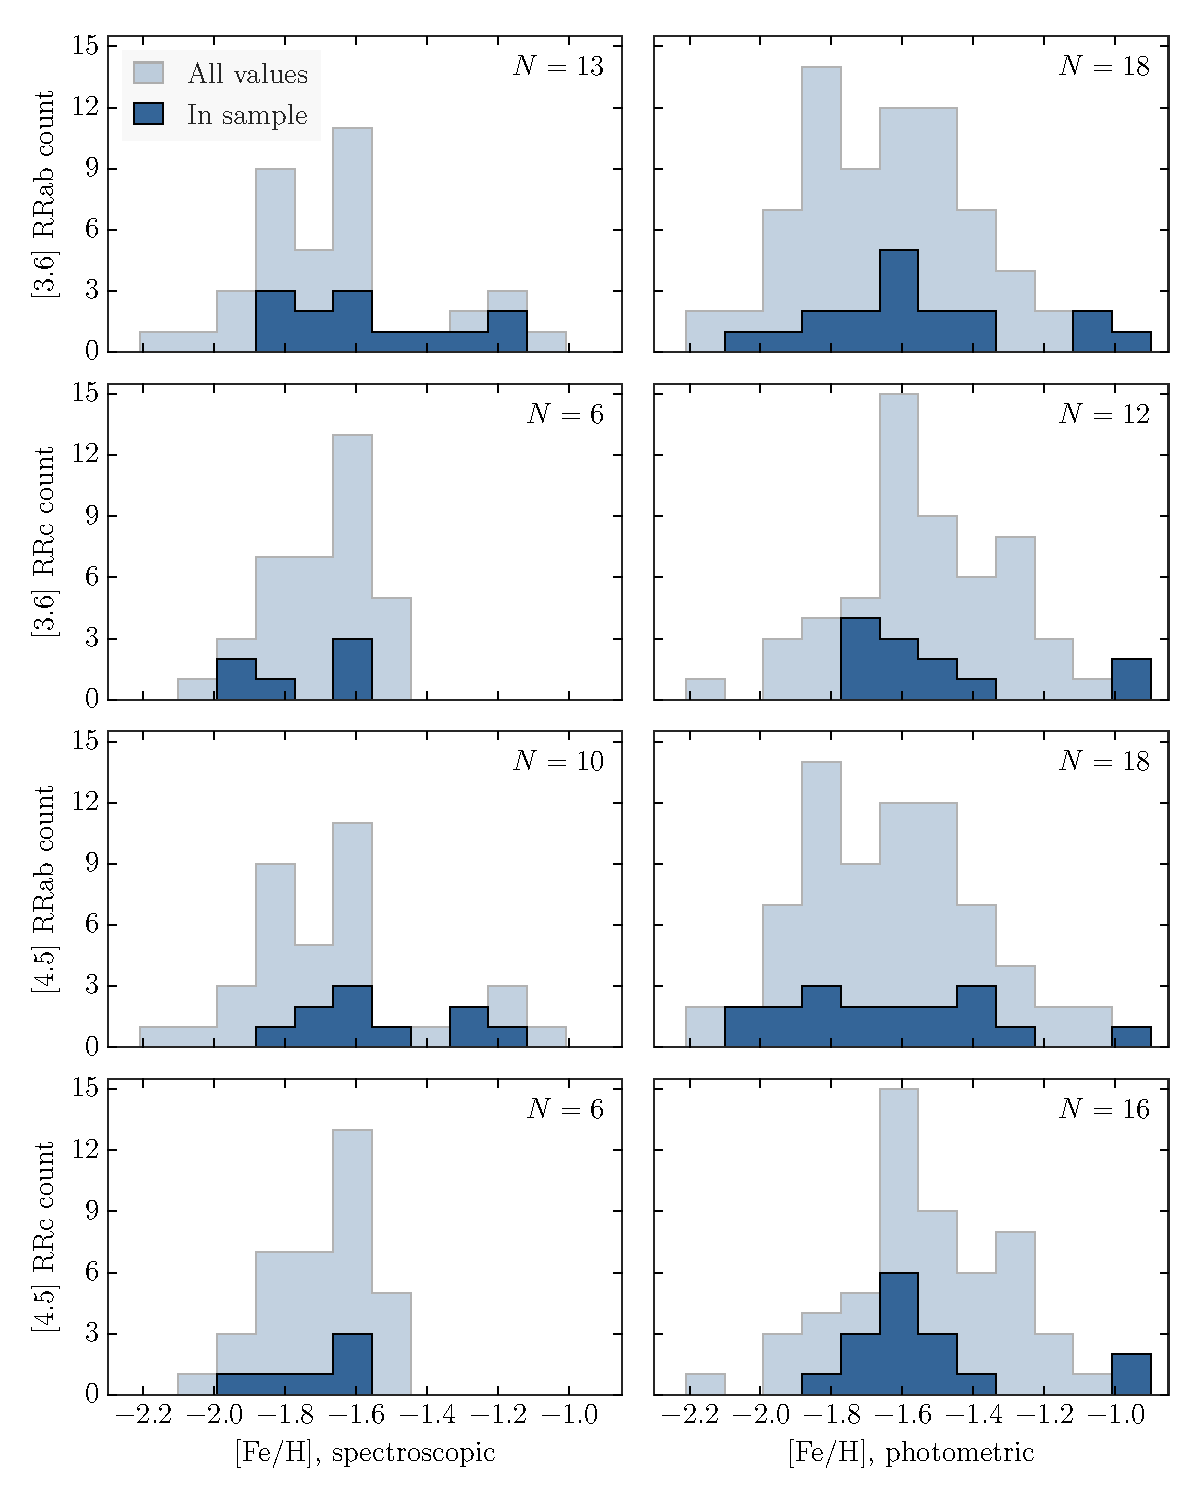
\includegraphics[width=160mm]{reworked_fitting_code/final_plots/metallicity_hists.pdf}
\caption{Histograms of spectroscopic \citep[left column]{2006ApJ...640L..43S} and photometric \citep[right column]{2000AJ....119.1824R} [Fe/H] values for RRab (top row) and RRc (bottom row). The light blue histograms represent all known metallicity values for each type, and the dark blue are the metallicity values for our final RRL sample in each passband. The number $N$ at the top right corner of each subplot is the number of stars in our final sample that have known metallicity values for the given type, wavelength, and metallicity catalog.}
\label{fig:metallicity_hists}
\end{center}
\end{figure*}

The fitted PL relations for all five bands are shown in Figure~\ref{fig:omegaCen_pl_m4}. Coloured points (purple, blue, green, yellow, red) represent the $J, H, K_S,$ [3.6], and [4.5] data that was included in the PL fits. Grey points represent stars that were excluded from the fits due to a lack of data in all bands; this ensured that the fits are done with a uniform sampling of all periods and metallicities. The two white points indicate stars which were rejected after the sigma clipping procedure described above. The distance moduli derived from these PL fits, uncorrected for extinction, are given in Table~\ref{tab:dist_mod}.

\begin{figure*}
\begin{center}
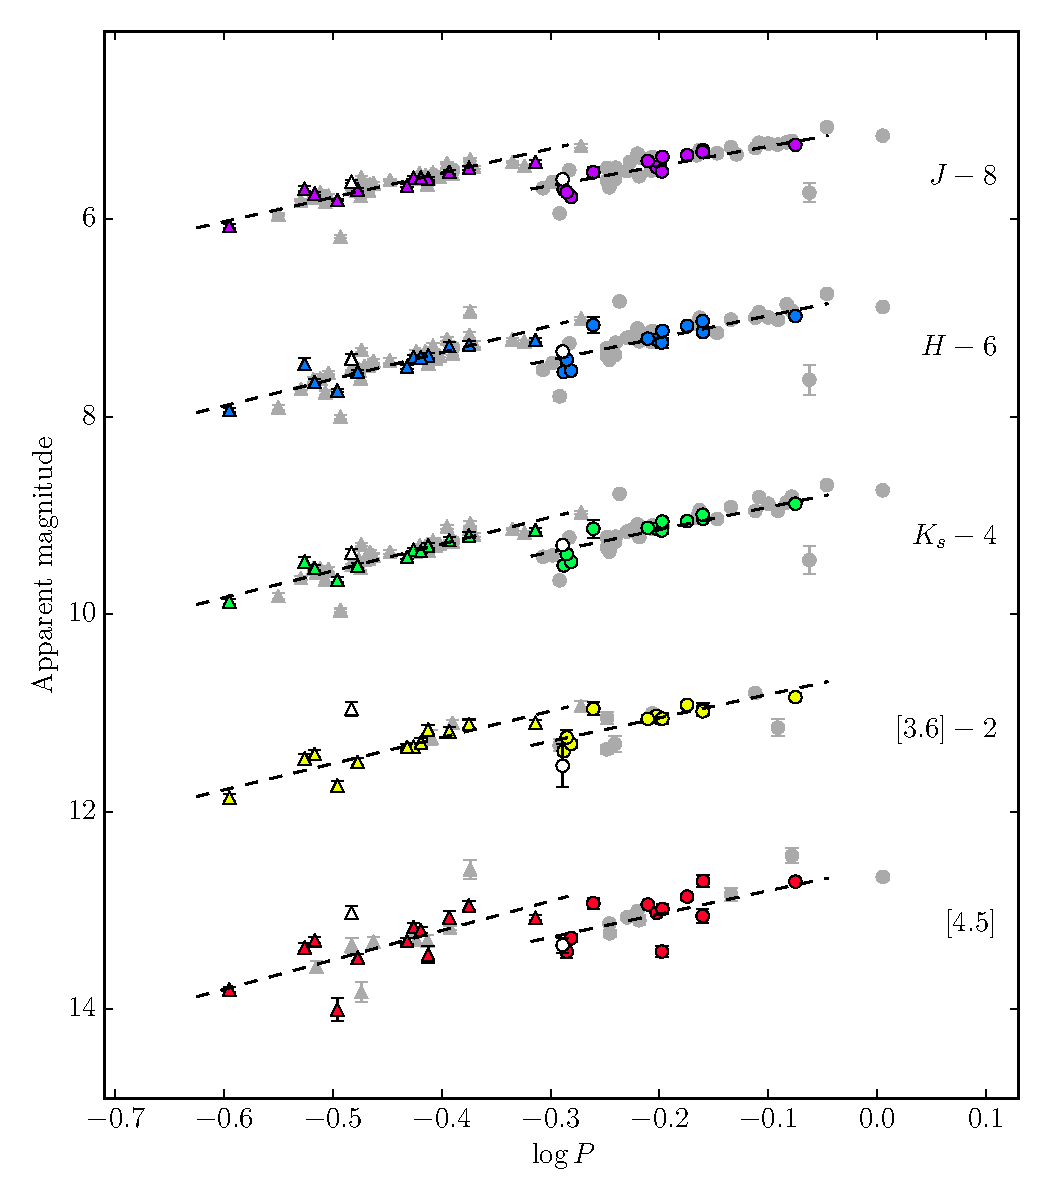
\includegraphics[width=160mm]{reworked_fitting_code/final_plots/multiwavelength_PL_m4_clipped.pdf}
\caption{PL relations for $J\!H\!K_s$, [3.6], and [4.5] photometry assuming [Fe/H]$=-1.677$. Here circles represent RRab stars and triangles represent RRc's. Coloured points are the final consistent sample with photometry in all 5 wavebands that are used for PL fitting. Grey points are stars that did not appear in all bands and are not used for PL fitting. The unfilled points are stars rejected from the final sample based on $2\sigma$ clipping of the PL residuals in [3.6], where sigma clipping was performed only on the consistent sample.}
\label{fig:omegaCen_pl_m4}
\end{center}
\end{figure*}


\section{Distance Moduli}
\label{sec:distance_moduli}

We combine the uncorrected distance moduli from each bandpass to obtain a mean reddening value and reddening-corrected distance modulus. We fit the near-infrared reddening law from \citet{1989ApJ...345..245C} to the $JHK_s$ data and the mid-infrared law from \citet{2005ApJ...619..931I} to [3.6] and [4.5] simultaneously, assuming a ratio of total to selective absorption $R_V = 3.1$. The resulting fit is shown in Figure~\ref{fig:omegaCen_dist_m4_mean}. We derive a mean dereddened distance modulus of $\langle \mu_0 \rangle = 13.789 \pm 0.018$ with $E(B-V) = 0.084 \pm 0.030$ using the weighted mean RRab + RRc distance moduli. The individual uncorrected distance moduli $\mu$, corrected distance moduli $\mu_0$, and PL residuals are shown in Table~\ref{tab:dist_mod}.

\begin{figure}
\begin{center}
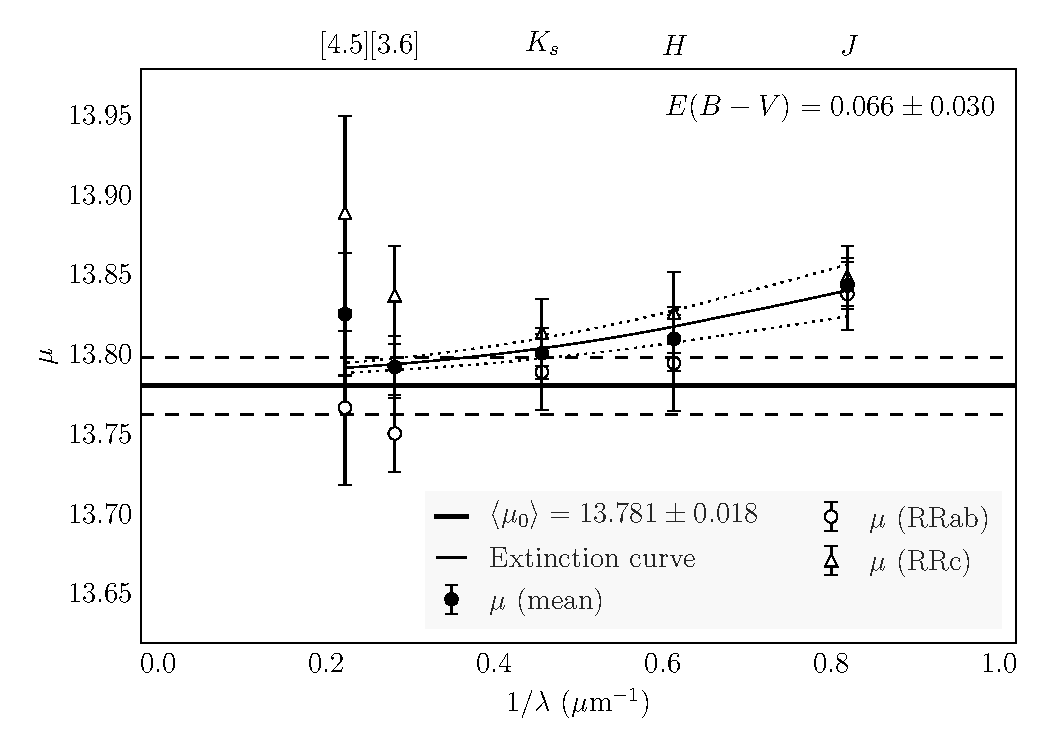
\includegraphics[width=80mm, trim=0.75cm 0 0.5cm 0]{reworked_fitting_code/final_plots/multiwavelength_distance_m4_clipped_mean.pdf}
\caption{Top: Uncorrected distance moduli for the final sample of $J\!H\!K_s$, [3.6], and [4.5] photometry. Filled circles are the mean distance moduli using both RRab and RRc stars, open circles are the distance moduli using only RRab stars, and open triangles are distance moduli using only RRc stars. Here the NIR and MIR reddening laws are fit to the mean distance moduli. The solid and dashed horizontal lines are the mean corrected distance modulus and its $1\sigma$ errors respectively. Bottom: reddening-corrected distance moduli and mean corrected distance modulus. Errors on the corrected distance moduli are the quadrature sum of the uncorrected distance moduli errors and the reddening error at the requisite wavelength.}
\label{fig:omegaCen_dist_m4_mean}
\end{center}
\end{figure}

\begin{figure}
\begin{center}
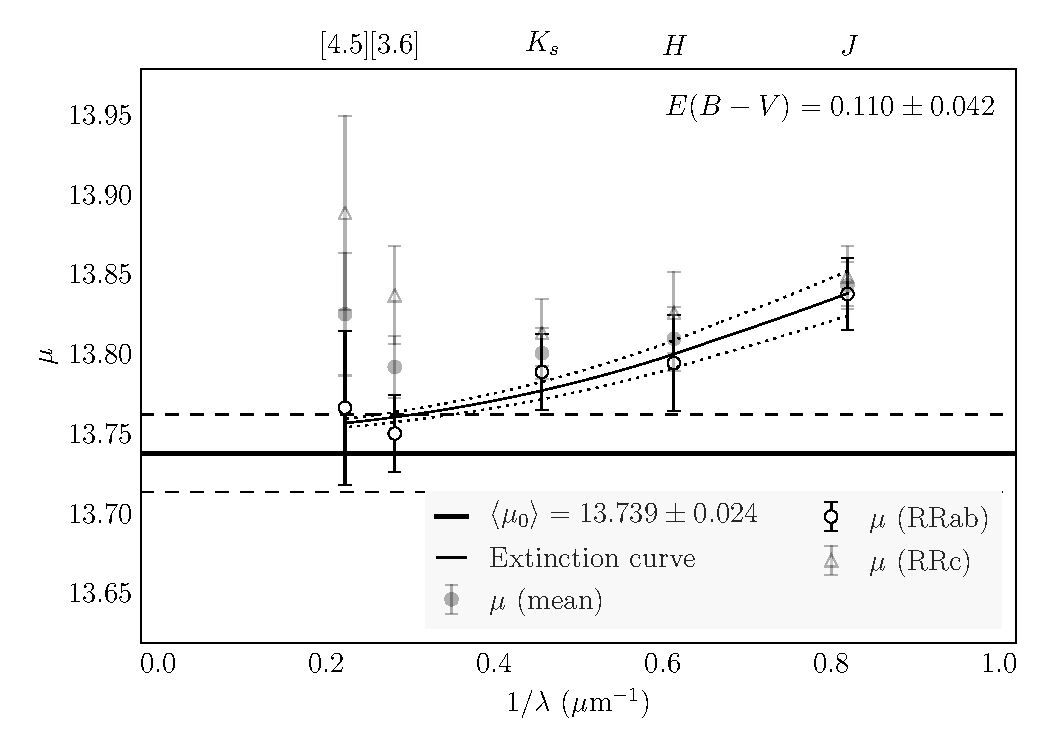
\includegraphics[width=80mm, trim=0.75cm 0 0.5cm 0]{reworked_fitting_code/final_plots/multiwavelength_distance_m4_clipped_ab.pdf}
\caption{Same as Figure~\ref{fig:omegaCen_dist_m4_mean}, with the reddening laws fit to the RRab distances only instead of the mean. RRc distance moduli and mean distance moduli are greyed out.}
\label{fig:omegaCen_dist_m4_ab}
\end{center}
\end{figure}

\begingroup
\setlength{\tabcolsep}{.5em}

\begin{table*}
\centering
\caption{Uncorrected distance moduli $\mu$, corrected distance moduli $\mu_0$, and the measured PL dispersion $\sigma$ for all wavelengths and pulsation modes. The corrected distance moduli $\mu_0$ are equal to $\mu - A_\lambda A_V$, where $A_V$ is derived from fitting the reddening laws to the mean distance moduli.}
\label{tab:dist_mod}
\begin{tabular}{l||c|c|c|c|c|c|c|c|r} 
\hline \hline
Band & $\mu$, RRab & $\mu$, RRc & $\mu$, RRab + RRc & $\mu_0$, RRab & $\mu_0$, RRc & $\mu_0$, RRab + RRc & $\sigma_{\text{PL}}$, RRab & $\sigma_{\text{PL}}$, RRc \\
\hline
$J$ & $13.865 \pm 0.023$ & $13.866 \pm 0.019$ & $13.865 \pm 0.015$ & $13.788 \pm 0.036$ & $13.790 \pm 0.033$ & $13.789 \pm 0.031$ & 0.127 & 0.082 \\
$H$ & $13.821 \pm 0.032$ & $13.844 \pm 0.026$ & $13.832 \pm 0.021$ & $13.773 \pm 0.037$ & $13.796 \pm 0.031$ & $13.784 \pm 0.027$ & 0.170 & 0.107 \\
$K_s$ & $13.816 \pm 0.025$ & $13.831 \pm 0.021$ & $13.824 \pm 0.016$ & $13.786 \pm 0.027$ & $13.801 \pm 0.024$ & $13.794 \pm 0.020$ & 0.147 & 0.089 \\
$[3.6]$ & $13.750 \pm 0.026$ & $13.838 \pm 0.031$ & $13.794 \pm 0.020$ & $13.733 \pm 0.027$ & $13.821 \pm 0.031$ & $13.777 \pm 0.021$ & 0.124 & 0.096 \\
$[4.5]$ & $13.771 \pm 0.052$ & $13.890 \pm 0.061$ & $13.830 \pm 0.040$ & $13.756 \pm 0.052$ & $13.875 \pm 0.061$ & $13.816 \pm 0.040$ & 0.154 & 0.219 \\
\hline
\end{tabular}
\end{table*}

\begin{comment}
$J$ & $13.865 \pm 0.023$ & $13.866 \pm 0.019$ & $13.865 \pm 0.015$ & $13.788 \pm 0.036$ & $13.790 \pm 0.033$ & $13.789 \pm 0.031$ & 0.127 & 0.082 \\
$H$ & $13.821 \pm 0.032$ & $13.844 \pm 0.026$ & $13.832 \pm 0.021$ & $13.773 \pm 0.037$ & $13.796 \pm 0.031$ & $13.784 \pm 0.027$ & 0.170 & 0.107 \\
$K_s$ & $13.816 \pm 0.025$ & $13.831 \pm 0.021$ & $13.824 \pm 0.016$ & $13.786 \pm 0.027$ & $13.801 \pm 0.024$ & $13.794 \pm 0.020$ & 0.147 & 0.089 \\
$[3.6]$ & $13.750 \pm 0.026$ & $13.838 \pm 0.031$ & $13.794 \pm 0.020$ & $13.733 \pm 0.027$ & $13.821 \pm 0.031$ & $13.777 \pm 0.021$ & 0.124 & 0.096 \\
$[4.5]$ & $13.771 \pm 0.052$ & $13.890 \pm 0.061$ & $13.830 \pm 0.040$ & $13.756 \pm 0.052$ & $13.875 \pm 0.061$ & $13.816 \pm 0.040$ & 0.154 & 0.219 \\

$[3.6]$ & RRab & 0.124 & 0.040 & 0.052 & 0.106 \\
$[3.6]$ & RRc & 0.096 & 0.079 & 0.044 & 0.034 \\
$[4.5]$ & RRab & 0.154 & 0.045 & 0.046 & 0.140 \\
$[4.5]$ & RRc & 0.219 & 0.057 & 0.054 & 0.205 \\
\end{comment}

\endgroup

\begin{table}
\centering
\caption{Corrected distance moduli $\mu_0$ using the $A_V$ value derived from fitting the reddening laws to only the RRab distance moduli.}
\label{tab:dist_mod_ab}
\begin{tabular}{l||c|c|c|r} 
\hline \hline
Band & $\mu_0$, RRab & $\mu_0$, RRc & $\mu_0$, RRab + RRc \\
\hline
$J$ & $13.739 \pm 0.047$ & $13.741 \pm 0.045$ & $13.740 \pm 0.043$ \\
$H$ & $13.742 \pm 0.041$ & $13.766 \pm 0.036$ & $13.754 \pm 0.033$ \\
$K_s$ & $13.767 \pm 0.030$ & $13.782 \pm 0.026$ & $13.775 \pm 0.023$ \\
$[3.6]$ & $13.722 \pm 0.028$ & $13.810 \pm 0.032$ & $13.766 \pm 0.022$ \\
$[4.5]$ & $13.747 \pm 0.053$ & $13.866 \pm 0.061$ & $13.806 \pm 0.041$ \\
\hline
\end{tabular}
\end{table}

\begin{comment}
& $13.739 \pm 0.047$ & $13.741 \pm 0.045$ & $13.740 \pm 0.043$ \\
& $13.742 \pm 0.041$ & $13.766 \pm 0.036$ & $13.754 \pm 0.033$ \\
& $13.767 \pm 0.030$ & $13.782 \pm 0.026$ & $13.775 \pm 0.023$ \\
& $13.722 \pm 0.028$ & $13.810 \pm 0.032$ & $13.766 \pm 0.022$ \\
& $13.747 \pm 0.053$ & $13.866 \pm 0.061$ & $13.806 \pm 0.041$ \\
\end{comment}

It is apparent from Figure~\ref{fig:omegaCen_dist_m4_mean} that there are large discrepancies in the distance moduli in [3.6] and [4.5] for the two pulsation modes; these discrepancies contribute to the relatively low $E(B-V)$ value and high dereddened distance modulus compared to previously determined values \citep[e.g.][]{2002ASPC..265...95L, 2006ApJ...652..362D}. % 0.11 and whatever the fuck distance moduli
If we remove the RRc's and fit the extinction curve only to the RRab's, as shown in Figure~\ref{fig:omegaCen_dist_m4_ab}, we obtain a better fit of all points to the extinction curve than when we use the mean. From these distance moduli we derive a dereddened distance modulus of $\langle \mu_0 \rangle = 13.743 \pm 0.026$ with $E(B-V) = 0.138 \pm 0.044$, both of which are closer to accepted values than the values derived from the weighted mean distance moduli. All individual corrected distance moduli from this fit are shown in Table~\ref{tab:dist_mod_ab}.

Given the large errors in the [4.5] distance moduli, we also fit the extinction curve to the $JHK_s$ and [3.6] distances only, excluding [4.5] entirely; this was found to have a negligible effect on the final derived distance modulus and reddening for both the mean and RRab-only measurements. %say what it is

% The distance moduli are plotted in fig blah for each wavelength
% cite smc paper for reddening fits

\section{Metallicity}
\label{sec:metallicity}

In principle, moving from the optical to the mid--infrared in uncrowded systems should bring the advantage of a steeper PL relation with decreased dispersion. However, theoretical works suggest that the metallicity coefficient in the infrared PL relations should be comparable to the metallicity coefficient at optical wavelengths \citep{2001MNRAS.326.1183B, 2004ApJS..154..633C, 2015ApJ...808...50M}. %"we can't send this out to Bono with that sentence in there" daaaamn
 $\omega$ Cen is ideal for assessing the contribution of metallicity to the mid--IR RRL PL relation, because it is known to have a large spread in metallicity \citep[$0.8~\leq~\Delta~\text{[Fe/H]}~\leq~1.4$~dex][]{2014ApJ...791..107V, 2012ApJ...746...14M, 2010ApJ...722.1373J}. A metallicity spread this wide is not found in any other Galactic globular cluster. 

One of the advantages of using globular clusters to calibrate PL coefficients is that all stars in a cluster can be considered to be at the same distance. The dispersion in the PL relation is a combination of the a) the intrinsic dispersion of the PL relation, b) the photometric uncertainties, and c) dispersion induced by other complicating factors such as the spread in metallicity. %Justify using M4 scatter - low crowding, whatever the fuck, copy overview paper
Since we have a measured ``intrinsic" dispersion of the RRL PL in [3.6] and [4.5] from the cluster M4 \citep{2015ApJ...808...11N} and the photometric uncertainties are well understood, we can isolate the remaining scatter due to astrophysical sources such as metallicity. 

It has been shown with mid-IR spectra that a significant CO feature sits within the IRAC [4.5] filter. In the case of Cepheids, \citet{2016MNRAS.tmp..421S} have shown that this has a significant effect on the [4.5] magnitudes, and is metallicity dependent. However, this effect decreases with increasing temperatures, turning off completely above 6000~K where all the CO has been destroyed \citep{2016MNRAS.tmp..421S}. As even the coolest RRL have temperatures over 6000~K \citep{1971PASP...83..697I}, we expect to see no such CO absorption affecting the [4.5] PL relation, nor do we expect any other temperature dependent (hence period dependent) metallicity effects. However, we can directly and empirically test this prediction. %If there are any other unanticipated metallicity effects for RRL, they must be smaller than the dispersion of the PL relations themselves, but we must still perform empirical tests to search for such effects.

\subsection{Metallicity Contribution to the Overall Dispersion}
\label{sec:dispersions}

We can place an upper limit on the contribution of metallicity to the $\omega$~Cen PL dispersion using the known variances of the individual components: the observed distribution of $\omega$~Cen PL residuals $\sigma_{\text{observed}}^2$, the intrinsic PL width $\sigma_{\text{intrinsic}}^2$, and the dispersion induced by photometric error $\sigma_{\text{phot}}^2$. The dispersion contributed by metallicity can therefore be constrained as follows:

\begin{equation}
\sigma_\text{[Fe/H]} \leq \sqrt{\sigma_{\text{observed}}^2 - \sigma_{\text{intrinsic}}^2 - \sigma_{\text{phot}}^2}
\end{equation}

%change vocab to overview paper - sig_astro, sig_meas, sig_int, sig_tot
%go through rachael's logic
%HOW ARE WE DEFINING INTRINSIC

Table~\ref{tab:metallicity_sigma} shows the estimated contribution to the dispersion from metallicity $\sigma_{[Fe/H]}$ in each band, alongside the contributions from the photometric uncertainties and intrinsic components \citep[from][for the near-- and mid--IR, respectively]{2015ApJ...808...50M, 2015ApJ...808...11N}. We note that this procedure is robust despite the inclusion of the metallicity term, $c$, in the near--IR PL relations (Equation~\ref{eqn:marconi_pl} and Table~\ref{tab:pl_table_theo}), as this is a constant term multiplied by a single [Fe/H] applied to each RRL uniformly, while the methodology described in this section studies the differential effects of the varying metallicities in \ocen.


\begin{table}
\centering
\caption{The standard deviation of the observed spread of the PL residuals $\sigma_{\text{observed}}$ ($\sigma_{\text{PL}}$ in Table~\ref{tab:dist_mod}) and its components: $\sigma_{\text{intrinsic}}$ ($\sigma$ in Table~\ref{tab:pl_table_m4}), $\sigma_{\text{phot}}$, and $\sigma_{[\text{Fe/H}]}$ for all PL relations.}
\label{tab:metallicity_sigma}
\begin{tabular}{lccccr} 
\hline \hline
Band & Mode & $\sigma_{\text{observed}}$ & $\sigma_{\text{intrinsic}}$ & $\sigma_{\text{phot}}$ & $\sigma_{[\text{Fe/H}]}$ \\
\hline
$J$ & RRab & 0.127 & 0.060 & 0.018 & 0.111 \\
  & RRc & 0.082 & 0.040 & 0.015 & 0.070 \\
$H$ & RRab & 0.170 & 0.040 & 0.028 & 0.163 \\
  & RRc & 0.107 & 0.020 & 0.024 & 0.102 \\
$K_s$ & RRab & 0.147 & 0.030 & 0.023 & 0.142 \\
  & RRc & 0.089 & 0.020 & 0.021 & 0.084 \\
$[3.6]$  & RRab & 0.124 & 0.040 & 0.052 & 0.106 \\
  & RRc & 0.096 & 0.079 & 0.044 & 0.034 \\
$[4.5]$& RRab & 0.154 & 0.045 & 0.046 & 0.140 \\
  & RRc & 0.219 & 0.057 & 0.054 & 0.205 \\
\hline
\end{tabular}
\end{table}
\begin{comment}
$[3.6]$ & RRab & 0.088 & 0.040 & 0.048 & 0.062 \\ %& $0.282$ & $0.234$\\
$[3.6]$ & RRc & 0.102 & 0.079 & 0.041 & 0.050 \\ %& $0.778$ & $0.323$\\
$[4.5]$ & RRab & 0.173 & 0.045 & 0.046 & 0.160 \\ %& $0.712$ & $0.590$\\
$[4.5]$ & RRc & 0.202 & 0.057 & 0.048 & 0.188 \\ %& $1.660$ & $0.689$\\
\end{comment}

We use these estimates of $\sigma_\text{[Fe/H]}$ to assess the $\gamma$ parameter for $\omega$~Cen, where 
\begin{equation} \label{eqn:gamma}
\gamma = \dfrac {\Delta \text{mag}} {\Delta [\text{Fe/H}]}\text{ mag dex} ^{-1}\text{,}
\end{equation}
similar to $\gamma$ used to quantify the effect of metallicity on the zero-point of the Cepheid PL relation \citep{1998ApJ...498..181K, 2009MNRAS.396.1287S}. Here we calculate $\gamma$ in units of mag~dex$^{-1}$ by dividing the standard deviation of the metallicity component of the PL scatter by the standard deviation of the metallicity distribution for both \citep{2006ApJ...640L..43S} and photometric \citep{2000AJ....119.1824R} metallicities; the results for each PL are shown in Table~\ref{tab:gamma}. We use all available metallicity values for each pulsation mode when taking the standard deviation, as we do not have metallicity values for all the stars in our samples, although the metallicity values we do have trace the overall metallicity distributions fairly well (see Figure~\ref{fig:metallicity_hists}).

It is important to note that these values presented in Tables~\ref{tab:metallicity_sigma} and \ref{tab:gamma} are upper limits, and as we will show in Sections~\ref{sec:residuals} and~\ref{sec:discussion}, the size of the effect that can be attributed to metallicity effects alone may be much smaller. 

%For [3.6] we find $\gamma \leq 0.455$ mag~dex$^{-1}$ for RRab's, and $\gamma \leq 0.237$ mag~dex$^{-1}$ for RRc's. These values are upper limits, and as we will show in Sections~\ref{sec:residuals} and~\ref{sec:discussion}, the size of the effect that can be attributed to metallicity effects alone may be much smaller. 


\begin{table}
\centering
\caption{Metallicity standard deviations and $\gamma$ values.}
\label{tab:gamma}
\begin{tabular}{lccccr} 
\hline \hline
Band & Mode & $\sigma_{\text{spect[Fe/H]}}$ & $\sigma_{\text{phot[Fe/H]}}$ & $\gamma_{\text{spect}}$ & $\gamma_{\text{phot}}$ \\
\hline
$J$ & RRab & 0.215 & 0.262 & 0.515 & 0.423 \\
  & RRc & 0.132 & 0.245 & 0.529 & 0.285 \\
$H$ & RRab & 0.215 & 0.260 & 0.760 & 0.627 \\
  & RRc & 0.132 & 0.245 & 0.773 & 0.416 \\
$K_s$ & RRab & 0.215 & 0.258 & 0.659 & 0.549 \\
  & RRc & 0.132 & 0.242 & 0.636 & 0.347 \\
$[3.6]$ & RRab & 0.232 & 0.275 & 0.455 & 0.385 \\
  & RRc & 0.145 & 0.266 & 0.237 & 0.129 \\
$[4.5]$ & RRab & 0.215 & 0.285 & 0.653 & 0.492 \\
  & RRc & 0.107 & 0.244 & 1.904 & 0.837 \\
\hline
\end{tabular}
\end{table}

\subsection{PL Residuals and Individual Metallicities}
\label{sec:residuals}

$\omega$~Cen provides a second approach to testing for a metallicity effect on the RRL PL relation. The cluster is well studied and many of its RRL have spectroscopic or photometric metallicities in the literature \citep[e.g.][]{2006ApJ...640L..43S, 2000AJ....119.1824R}. 

Theory predicts a linear metallicity term in the PLZ relation in the optical and infrared, $c\times[\text{Fe/H}]$.
We thus fit a relation of the form
\begin{equation}
\label{eqn:delta_mag}
\Delta\text{mag} = \gamma \times[\text{Fe/H}] + d
\end{equation}
to the [3.6] and [4.5] PL residuals and metallicity values for stars with known metallicity values, as shown in Figures~\ref{fig:metallicity_residuals_3}, \ref{fig:metallicity_residuals_4},  \ref{fig:metallicity_residuals_j}, \ref{fig:metallicity_residuals_h}, and \ref{fig:metallicity_residuals_k}. The scatter in the [3.6] and [4.5] PL relations is higher for $\omega$~Cen than it is for M4 \citep{2015ApJ...808...11N, 2015ApJ...799..165B}; however, when we examine [Fe/H] vs. the residuals of each PL relation, $\gamma$ is within $2\sigma$ of zero for all fits, indicating that there is no significant metallicity dependence in the PL residuals. The flatness of these relations hints that the source of additional dispersion in the $\omega$~Cen PL relations may not be due to metallicity, but in fact due to other evolutionary effects such as the spread in age of its multiple populations. This is discussed further in Section~\ref{sec:discussion}.

However, the dominant source of uncertainty in these fits is the metallicity measurements, with typical errors approaching $\sim 0.5$~dex, and systematic offsets between the photometric and spectroscopic systems that make them unsuitable for use as one catalogue. More accurate metallicities will be required to constrain any potential effect more precisely.

\begin{figure*}
\begin{center}
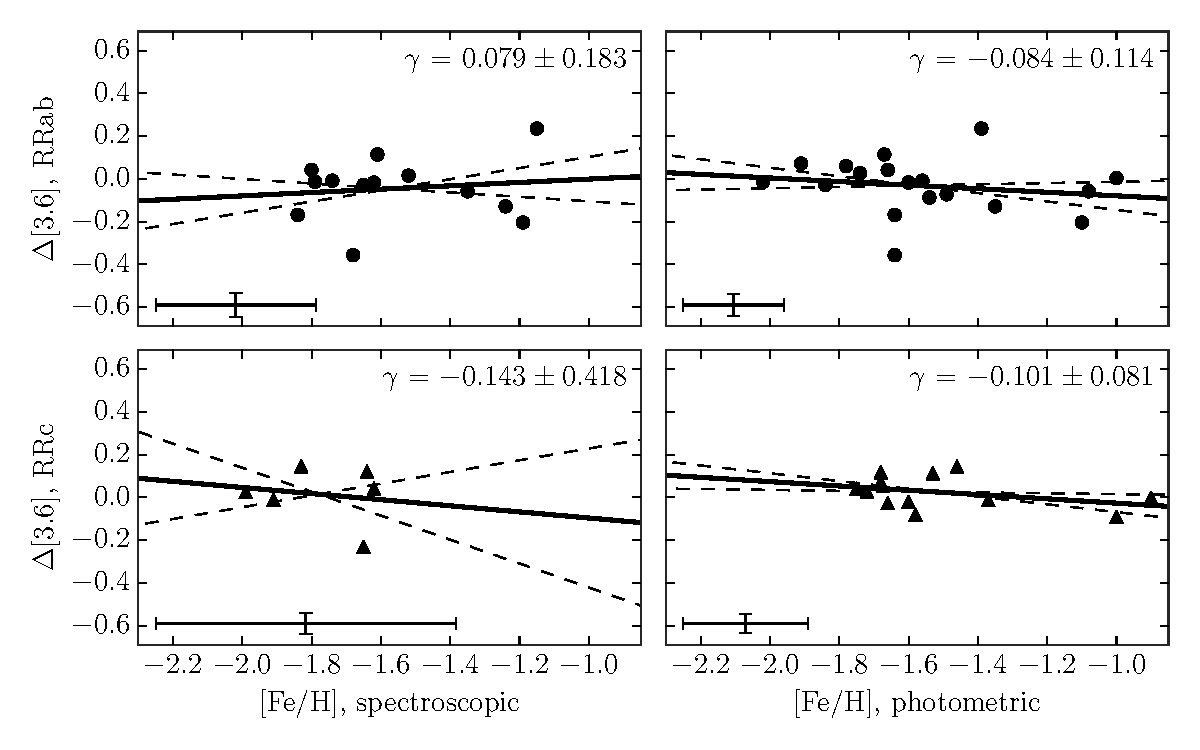
\includegraphics[width=160mm]{reworked_fitting_code/final_plots/metallicity_vs_residuals_3.pdf}
\caption{Spectroscopic \citep[left column]{2006ApJ...640L..43S} and photometric \citep[right column]{2000AJ....119.1824R} [Fe/H] values vs. period-luminosity residuals for RRab (top row) and RRc (bottom row) in [3.6]. Solid lines are the line of best fit with slope $\gamma$, and dashed lines are the $1\sigma$ confidence intervals. The crossed lines at the bottom left corner of each subplot represent average errors in [Fe/H] and $\Delta$mag. The $\gamma$ parameter from equation 4 is shown in the top right corner of each subplot. All $\gamma$ values are consistent with zero within $2\sigma$, and most are consistent within $1\sigma$.}
\label{fig:metallicity_residuals_3}
\end{center}
\end{figure*}

\begin{figure*}
\begin{center}
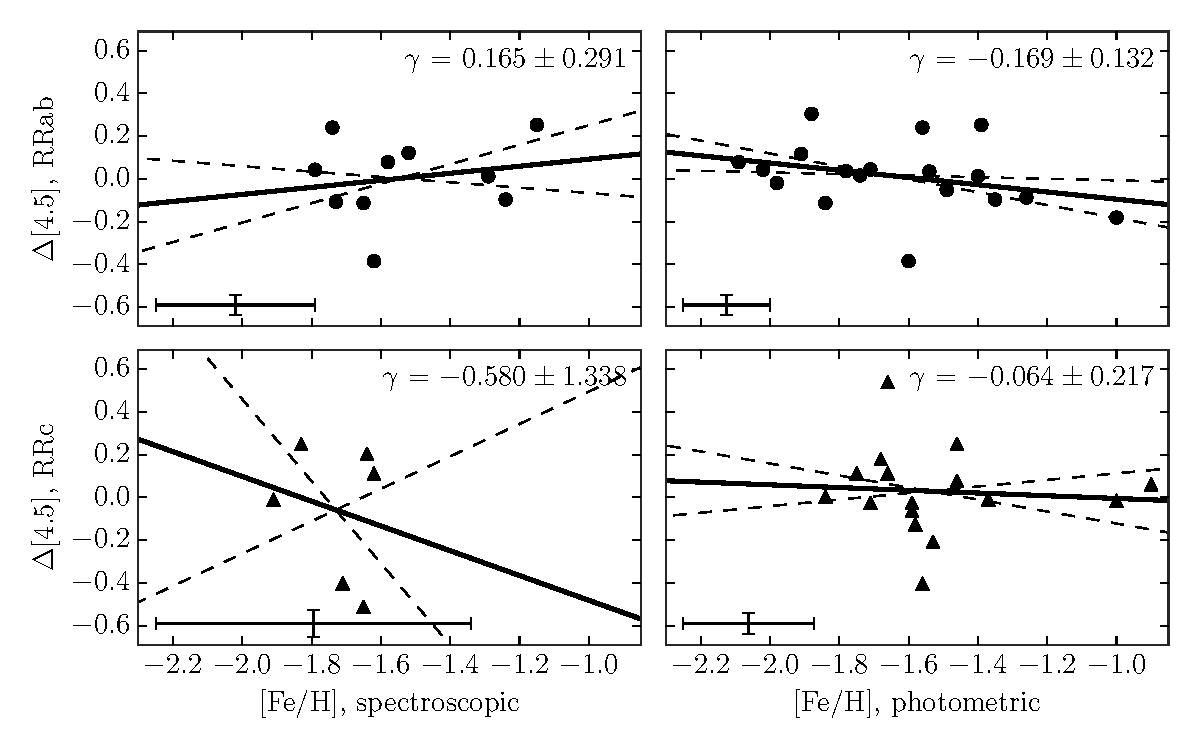
\includegraphics[width=160mm]{reworked_fitting_code/final_plots/metallicity_vs_residuals_4.pdf}
\caption{Same as Figure~\ref{fig:metallicity_residuals_3}, but for [4.5].}
\label{fig:metallicity_residuals_4}
\end{center}
\end{figure*}

\begin{figure*}
\begin{center}
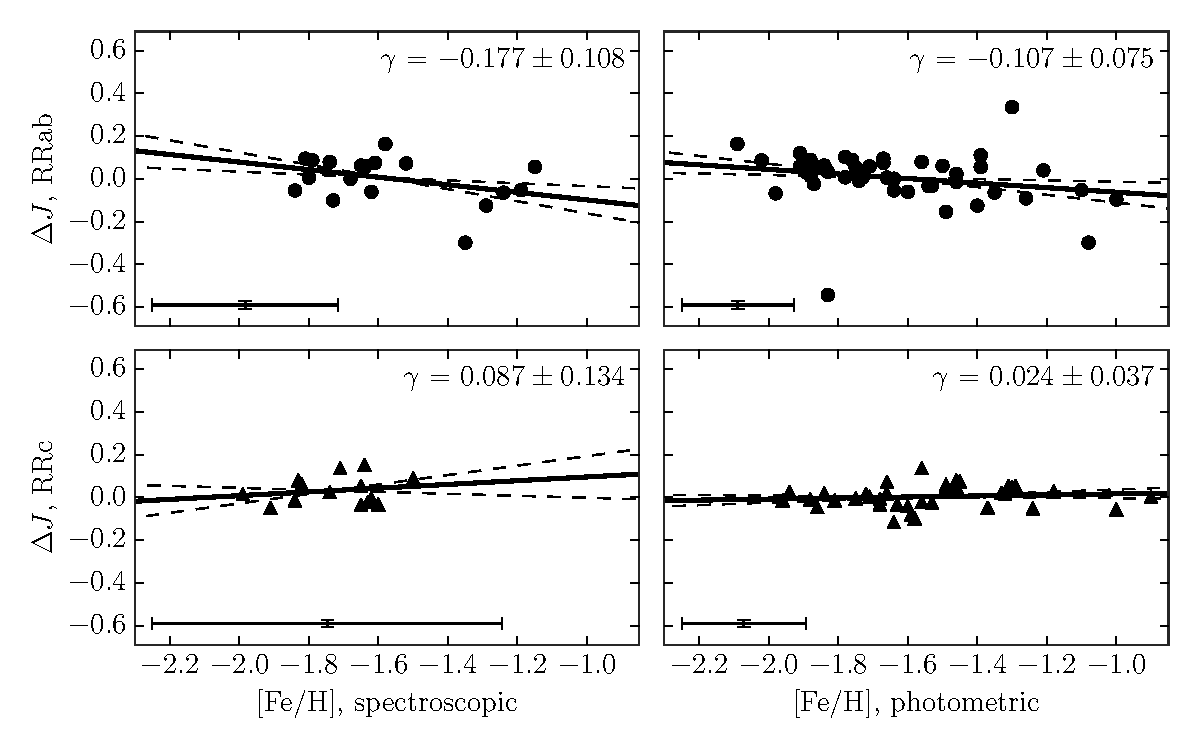
\includegraphics[width=160mm]{reworked_fitting_code/final_plots/metallicity_vs_residuals_J.pdf}
\caption{Same as Figure~\ref{fig:metallicity_residuals_3}, but for $J$.}
\label{fig:metallicity_residuals_j}
\end{center}
\end{figure*}

\begin{figure*}
\begin{center}
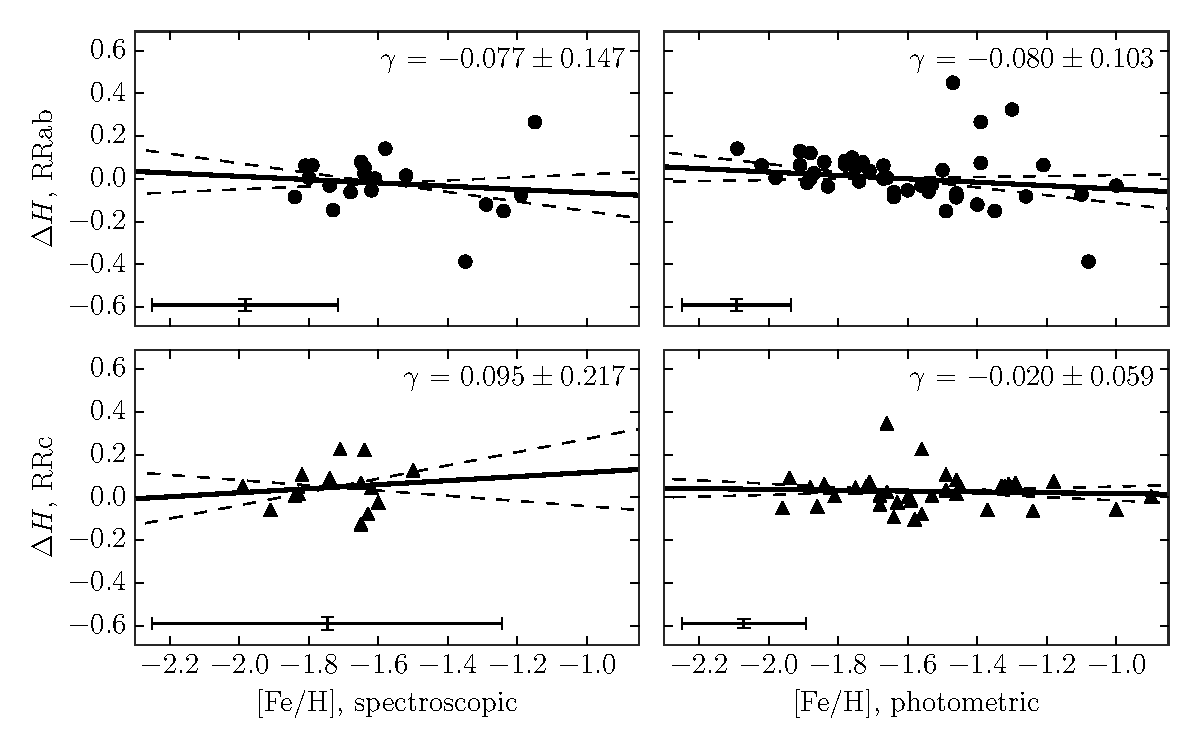
\includegraphics[width=160mm]{reworked_fitting_code/final_plots/metallicity_vs_residuals_H.pdf}
\caption{Same as Figure~\ref{fig:metallicity_residuals_3}, but for $H$.}
\label{fig:metallicity_residuals_h}
\end{center}
\end{figure*}

\begin{figure*}
\begin{center}
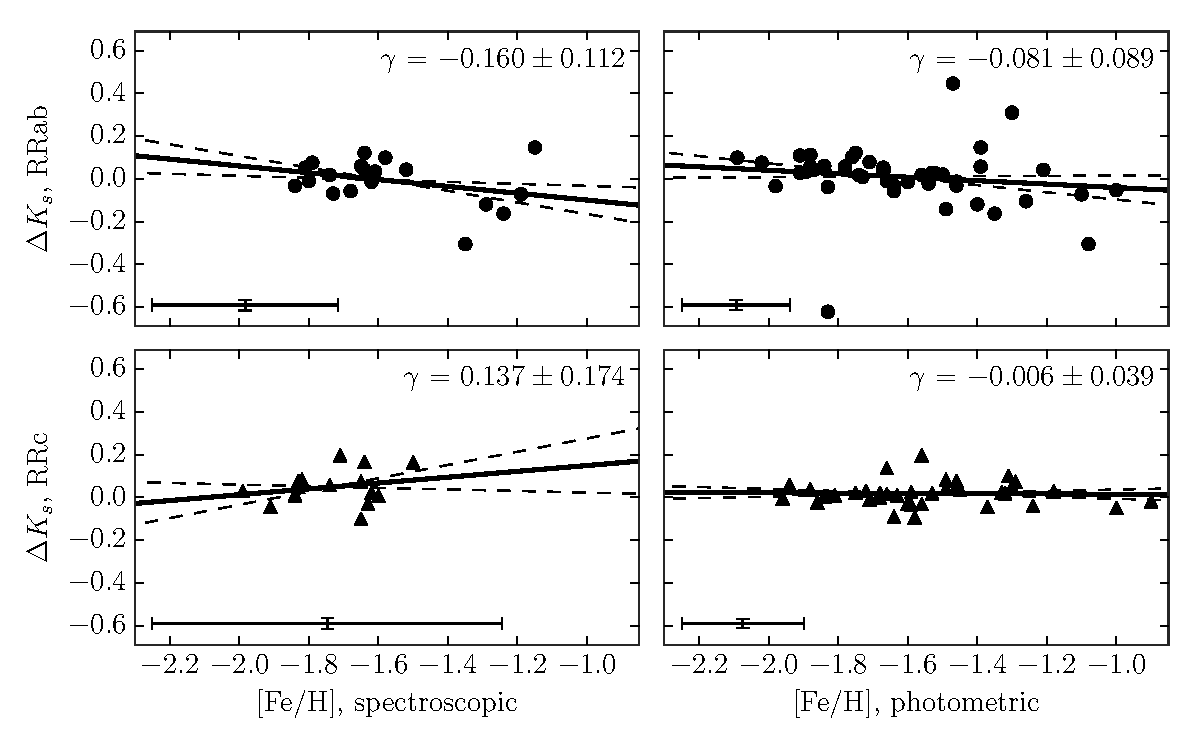
\includegraphics[width=160mm]{reworked_fitting_code/final_plots/metallicity_vs_residuals_K.pdf}
\caption{Same as Figure~\ref{fig:metallicity_residuals_3}, but for $K_s$.}
\label{fig:metallicity_residuals_k}
\end{center}
\end{figure*}

\begin{figure}
\begin{center}
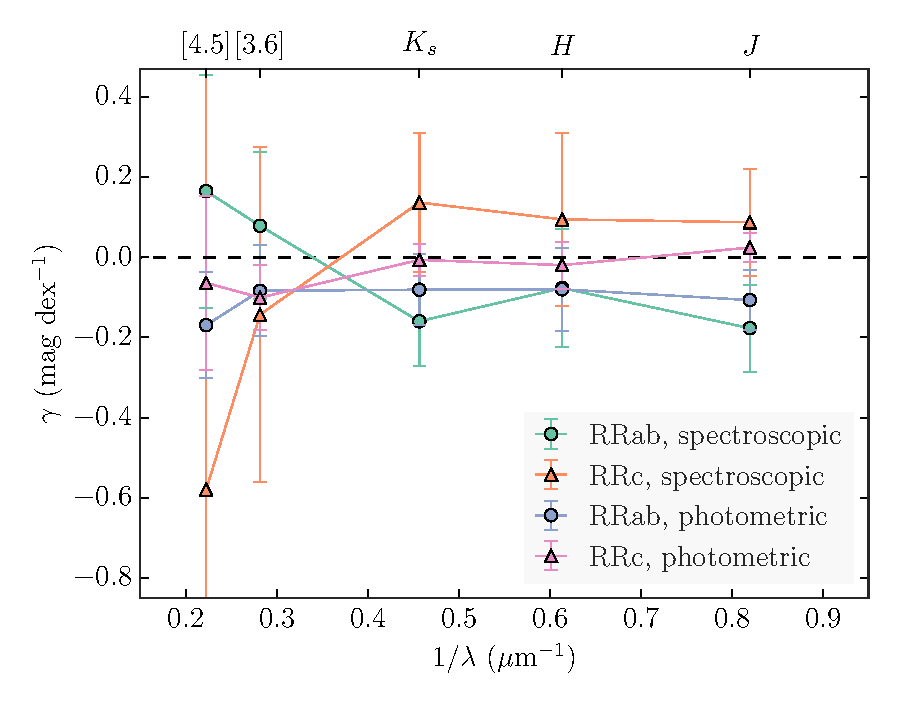
\includegraphics[width=80mm, trim=0.75cm 0 0.5cm 0]{reworked_fitting_code/final_plots/metallicity_slope_vs_wavelength.pdf}
\caption{Metallicity slope dependence on wavelength. At each of five
wavelengths along the x axis (corresponding to the $J$, $H$, $K$, 3.6 and 
4.5~$\mu$m bandpasses) we plot on the y axis the results of a
regression of magnitude residuals against metallicities, searching
both for a signal and for any trend in that signal with
wavelength. Neither trend is found. Colour--coded symbols break the data
down into RRab and RRC type variables (circles and triangles,
respectively) and into spectroscopically determined metallicities and
photometric metallicities (black/blue and red/green, respectively.)
Virtually all of the individual data points are consistent with no
metallicity effect on the observed magnitudes, independent of
wavelength, RRL type and/or metallicity determination method.}
\label{fig:metallicity_slopes}
\end{center}
\end{figure}


%\begin{comment}

%\end{comment}

\section{Discussion}
\label{sec:discussion}

\begin{comment}
\begin{figure}
\begin{center}
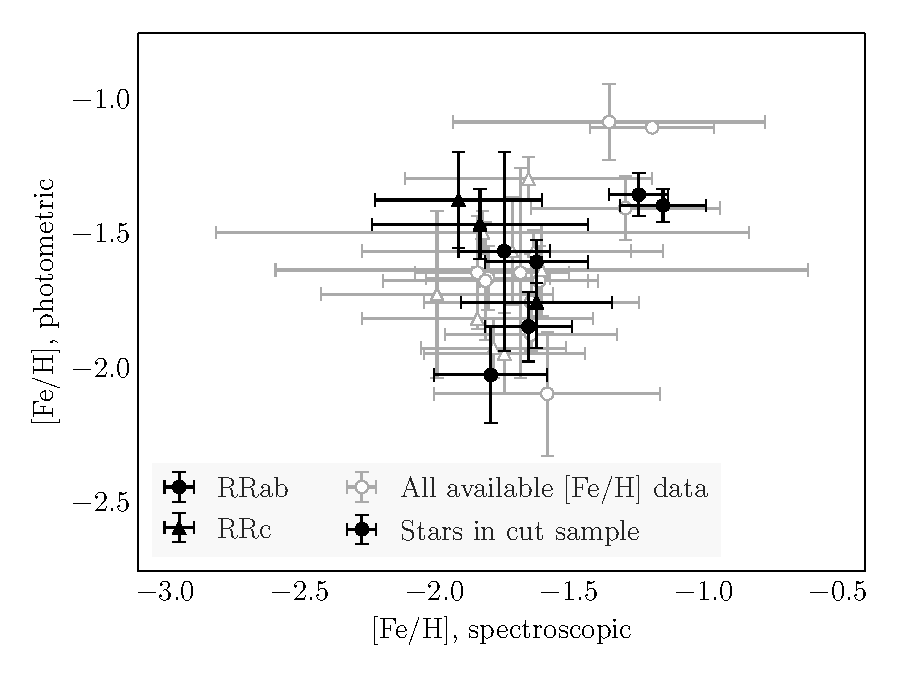
\includegraphics[width=80mm]{reworked_fitting_code/final_plots/metallicity_comparison_all_clipped.pdf}
\caption{Spectroscopic vs. photometric measurements of [Fe/H] for RRLs in $\omega$~Cen.}
\label{fig:metallicity_comparison}
\end{center}
\end{figure}
\end{comment}

% 1. Add discussion of why gamma in 6.1 is big but gamma in 6.2 is small Ñ age/mass spread rather than metallicity effect. Can refer to new plot here too.

% 2. Why the discrepancy between RRab and RRc - data effect rather than intrinsic??

\subsection{Evolutionary Effects}
\label{sec:evolution}
While we find high upper bounds on the contribution of metallicity to the PL scatter in all infrared passbands, it is unlikely that this scatter is due to metallicity alone. \citet{1986A&A...169..111G} and \citet{1991ApJ...373L..43L} demonstrate that RRL luminosity is dependent on the horizontal branch morphology as well as metallicity; it is also well known that $\omega$~Cen contains RRLs in multiple evolutionary states \citep{2008MmSAI..79..342S, 2015A&A...577A..99N}.

\citet{2015ApJ...808...50M} performed extensive theoretical studies of the effects of both RRL composition and evolutionary state on the position of the horizontal branch in the Hertzsprung--Russell (HR) diagram. In their figure 2 they present the HR diagram for a selection of models at a fixed composition for a range of evolutionary states, demonstrating a spread in 0.3~dex in bolometric luminosity between the least evolved, zero--age horizontal branch (ZAHB) mass RRL and the most evolved RRL. The RRL population in $\omega$~Cen is thought to be comprised of (at least) two different populations --- the metal rich population being the less evolved ZAHB phase stars, with the more metal poor population in an advanced evolutionary state \citep{2016MNRAS.457.4525T}. This spread in evolutionary state \textit{in addition to} the spread in metallicity could create the additional dispersion observed in the $\omega$~Cen PL relations. 

Figures~\ref{fig:hband_spectro} and~\ref{fig:hband_photo} demonstrate the need for an additional evolutionary parameter. Both the $H$ and [3.6] bands show additional scatter in the $\omega$~Cen PL relations above that which can be explained by the intrinsic dispersion and photometric uncertainties alone. Figures~\ref{fig:hband_spectro} and~\ref{fig:hband_photo} show the PL relations with the stars colour coded by metallicity. If metallicity were the dominant factor in the additional dispersion we would expect that the high metallicity points would sit on one side of the mean PL, with the low metallicity points on the other. This is not the case in either the $H$ or [3.6] bands; the metallicities appear to be randomly distributed about the mean PLs. This is a clear suggestion that the dominant effect contributing to the dispersion in the  $\omega$~Cen PL relation is a spread in evolutionary state (i.e. age), rather than composition. 

\begin{figure*}
\begin{center}
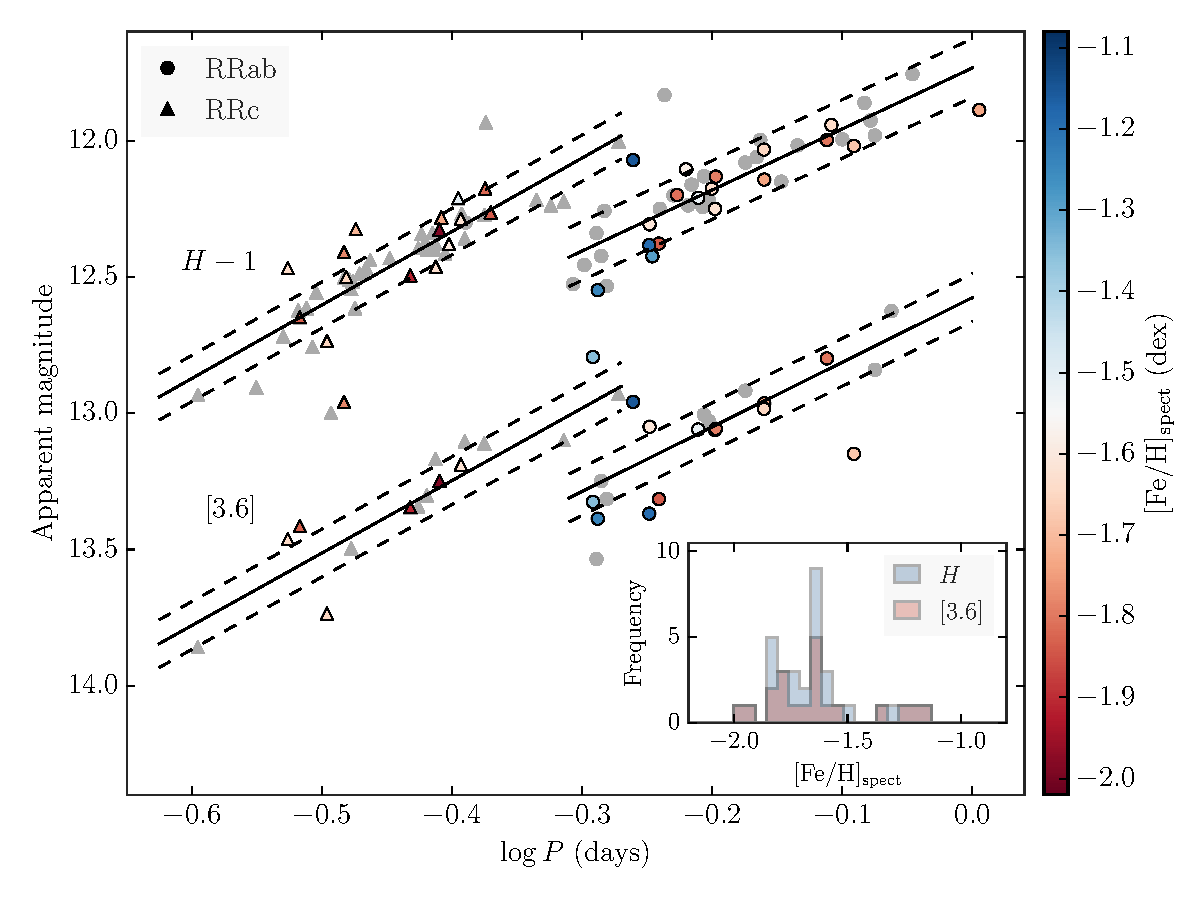
\includegraphics[width=160mm]{reworked_fitting_code/final_plots/spect_color_PL.pdf}
\caption{$H$ and [3.6] PL relations, with colour indicating spectroscopic \citep{2006ApJ...640L..43S} metallicity values. Grey points have no known metallicity values. There is no trend between direction of deviation from the PL with metallicity in either the $H$ or [3.6] relation, demonstrating that the increased dispersion must have an additional evolutionary component.}
\label{fig:hband_spectro}
\end{center}
\end{figure*}

\begin{figure*}
\begin{center}
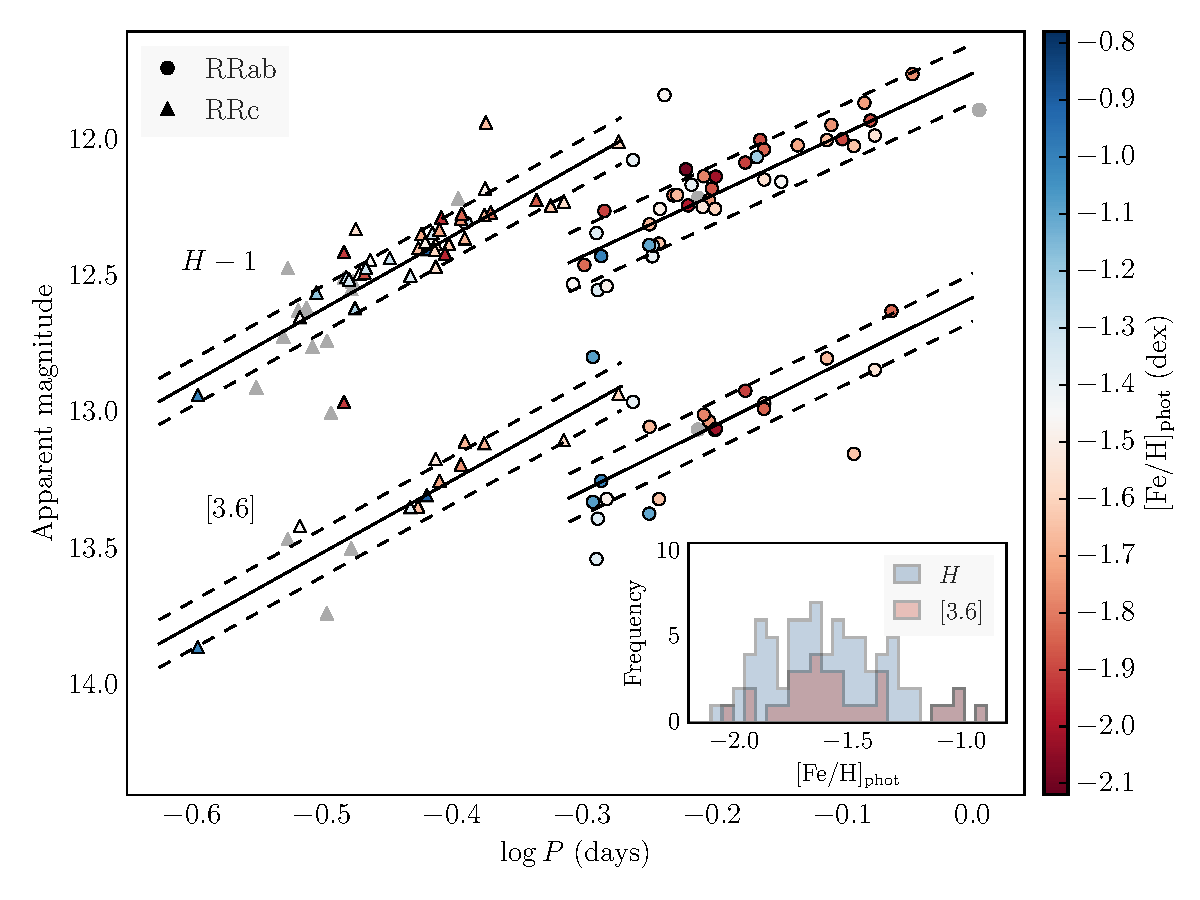
\includegraphics[width=160mm]{reworked_fitting_code/final_plots/phot_color_PL.pdf}
\caption{$H$ and [3.6] PL relations, with colour indicating photometric \citep{2000AJ....119.1824R} metallicity values. Grey points have no known metallicity values. There is no trend between direction of deviation from the PL with metallicity in either the $H$ or [3.6] relation, demonstrating that the increased dispersion must have an additional evolutionary component.}
\label{fig:hband_photo}
\end{center}
\end{figure*}

\subsection{Improvements to the Mid--IR PL Calibration}
\label{sec:improvements}
We note here a concern with the current adopted slopes for RRab and RRc variables at 4.5~$\mu$m from \citet{2015ApJ...808...11N} (and to a lesser degree for the corresponding slopes for the 3.6~$\mu$m PL relations). There are two indications that the slopes may not be correct. First, we note that the slope of the respective PL relations as a function of wavelength is not monotonically increasing with increasing wavelength, as expected as the slope asymptotically approaches the slope of the wavelength-independent period-radius relation. For the RRab variables a relatively smooth trend is observed. However, for the RRc
variables the situation is less clear. While the three near-infrared slopes follow the RRab trend in lock--step, the slope at 3.6~$\mu$m is very shallow with respect to the value expected from a smooth extrapolation from the shorter wavelengths, and then at 4.5~$\mu$m the
slope becomes unexpectedly large. This pattern of behaviour is unphysical. 

Future data, beyond the scope of this paper, will be required to improve upon these slopes; however, we note that the slopes at 3.6~$\mu$m and 4.5~$\mu$m should both be around $-2.80$, suggesting that 3.6~$\mu$m will be steeper by 0.09 (a 5\% adjustment) and that the slope at 4.5~$\mu$m  will be flatter by 0.18 (an 6\% adjustment). Second, the correspondence of the 3.6 and 4.5~$\mu$m magnitude residuals from their respective PL relations would be made tighter if the 4.5~$\mu$m PL relation for the RRc variables were made shallower, or the 3.6~$\mu$m slope made steeper, or both, as suggested above.

The issue of whether this difference in slope is due to differences in metallicity between \ocen and M4 \citep[the calibrating sample in][]{2015ApJ...808...11N}, or to another effect such as the discrepant period distributions of the samples, or a difference in analysis technique, requires an independent sample of RRL at a single metallicity, and as such cannot be answered with the \ocen sample. 

Results from the Gaia mission \citep{1996A&AS..116..579L} are expected to improve the overall characterisation of the RRL PL relation dramatically. Trigonometric parallaxes and spectrophotometric metallicities of Galactic RRLs from Gaia will increase the number of high quality calibrators for the infrared PL relations by an order of magnitude \citep[Scowcroft et al. 2016b, in prep., Beaton et al. 2016, in prep.]{2012MNRAS.426.2463L}. 

In addition to the calibration of the slope and absolute zero--point of the RRL PL relation, Gaia will also provide important insights regarding $\omega$~Cen. Gaia will observe many of the RRL in $\omega$~Cen \citep{2002ASPC..265..415B}, providing 0.2\% parallaxes and spectrophotometric metallicities for the individual stars. Combining the photometric data presented here with the Gaia sample of high--quality parallaxes and consistent metallicities we will be able to further constrain the effect on the mid--IR PL relation.

We also anticipate that the NIRCam instrument on {\em JWST} \citep{2005SPIE.5904...21B, 2006SSRv..123..485G} will provide substantial improvements over IRAC for investigations of this nature. The NIRCam filters F356W and F444W will provide data in passbands comparable to IRAC's [3.6] and [4.5] at an order of magnitude higher resolution (0.065 arcsec/pixel), which will significantly decrease photometric error due to crowding and therefore allow us to obtain data for the full sample of RRL in $\omega$~Cen. With the parallaxes and differential metallicities from Gaia, and the high precision photometry from {\it JWST}, studies of $\omega$~Cen will allow us to explore the effects of metallicity and evolutionary effects on the RRL populations of globular clusters. 

% 1. Add discussion of why gamma in 6.1 is big but gamma in 6.2 is small Ñ age/mass spread rather than metallicity effect. Can refer to new plot here too.

% 2. Why the discrepancy between RRab and RRc - data effect rather than intrinsic??

% 2015A&A...577A..99N 

% Eric Persson's metallicity omega cen project - 'we explore a subset of RR Lyrae variables in the w Centauri globular cluster for which a large set of stellar metallicities will be available for a broad range of RR Lyrae' overview paper
% spectroscopically with magellan

% zpt changes by .15 mag depending on whether you include RRc in galactic calibrator sample so ?????

\begin{comment}

Suggestions from what we discussed today:

* How does the choice of metallicity affect the results?
* Comparison of the photometric and spectroscopic metallicities - discussion of Fig 5
Ñ Also note figures must appear in the order they are referred to in the text.
* Could crowding have affected the result? Probably not systematically, BUT it did reduce the sample of RRL dramatically.
* How does the calibration of the PL affect the result?
* Better Calibration of the PL relation
* Future metallicity measurements
** GAIA
* Better resolution in the midÑIR
** JWST
VS will send references for GAIA, JWST separately

\end{comment}

\section{Conclusions}
\label{sec:conclusions}

We derive a mean dereddened distance modulus for $\omega$~Cen of ${\langle \mu_0 \rangle = 13.743 \pm 0.026}$ with reddening ${E(B-V) = 0.138 \pm 0.044}$ using distance moduli derived from RRab PL relations in $JHK_s$, [3.6], and [4.5]. Using the mean of RRab and RRc distance moduli in the same passbands, we derive a mean dereddened distance modulus of ${\langle \mu_0 \rangle = 13.789 \pm 0.018}$ with reddening ${E(B-V) = 0.084 \pm 0.030}$. The value found using RRab alone is in better agreement with those in the literature \citep[e.g.][]{2002ASPC..265...95L, 2006ApJ...652..362D}.

We also constrain the contribution of metallicity on the dispersion of the RRL PL relations by considering the variances associated with each component of the PL relation. We find that at most metallicity contributes 0.106 and 0.140~mag in dispersion to the [3.6] and [4.5] RRab PL relations respectively. Converting these values into $\gamma$, the PL relation metallicity coefficient, we find high upper limits compared to theoretical predictions for all infrared wavelengths. 

When deriving $\gamma$ empirically using the residuals from the RRL PL relations and the individual metallicities of the stars, we find $\gamma$ values consistent with zero at all infrared wavelengths. We thus conclude that the upper limits derived in Section~\ref{sec:dispersions} are likely a combination of metallicity and evolutionary effects due to the evolutionary spread of the populations in $\omega$~Cen.  

%, quantified as $\gamma = \Delta \text{mag} / \Delta [\text{Fe/H}]$, to the scatter of the $\omega$~Cen PL relations by subtracting the variances of the intrinsic scatter and photometric error from the observed PL variance and taking the square root of the result, and dividing that by the standard deviation of the distribution of metallicity values. We also measure $\gamma$ directly using the slope of the linear fit to the PL residuals vs. [Fe/H].

\section*{Acknowledgements}
\label{sec:acknowledgements}

We thank Eric Persson for his many contributions to this project.

This work is based on observations made with the Spitzer Space Telescope, which is operated by the Jet Propulsion Laboratory, California Institute of Technology under a contract with NASA. Support for this work was provided by NASA through an award issued by JPL/Caltech.

This work was also supported in part by the Claremont-Carnegie Astrophysics Research Program.

This publication makes use of data products from the Two Micron All Sky Survey, which is a joint project of the University of Massachusetts and the Infrared Processing and Analysis Center/California Institute of Technology, funded by the National Aeronautics and Space Administration and the National Science Foundation.

This research has made use of the NASA/IPAC Extragalactic Database (NED), which is operated by the Jet Propulsion Laboratory, California Institute of Technology, under contract with the National Aeronautics and Space Administration.


%%%%%%%%%%%%%%%%%%%%%%%%%%%%%%%%%%%%%%%%%%%%%%%%%%

%%%%%%%%%%%%%%%%%%%% REFERENCES %%%%%%%%%%%%%%%%%%

% The best way to enter references is to use BibTeX:

\bibliographystyle{mnras}
\bibliography{omegaCen_mnras_2016_vs}
 % if your bibtex file is called example.bib


% Alternatively you could enter them by hand, like this:
% This method is tedious and prone to error if you have lots of references

%%%%%%%%%%%%%%%%%%%%%%%%%%%%%%%%%%%%%%%%%%%%%%%%%%

%%%%%%%%%%%%%%%%% APPENDICES %%%%%%%%%%%%%%%%%%%%%

\clearpage
%\begin{comment}

\newpage

\appendix

%% To get the appendix table numbering right you need to have a section after the appendix command. This way the table will be referred to as Table A1, rather than Table 1 (which you already have another one of in the main text).

% Add comments to table
\setlength{\tabcolsep}{.5em}

\section{RRL Photometry}
\label{sec:phot_table_appendix}
\onecolumn
\begin{landscape}
\begin{center}
\scriptsize{
\begin{longtable}{lcccccccccccccccccccr}
\caption{Parameters for 99 RRLs in $\omega$~Cen. First five columns are star ID, right ascension and declination, pulsation mode, and period in days from \citet{2004A&A...424.1101K}. Columns 6 through 11 are $J\!H\!K_s$ apparent magnitudes and errors from FourStar data. Columns 12 through 17 are 3.6~$\mu$m and 4.5~$\mu$m apparent magnitudes, errors, and PL residuals ($\Delta [3.6]$ and $\Delta [4.5]$) from IRAC data. Columns 18-21 are photometric ([Fe/H], p) and spectroscopic ([Fe/H], s) metallicities and errors from \citet{2000AJ....119.1824R} and \citet{2006ApJ...640L..43S} respectively.
\label{tab:everything}} 
\tabularnewline 
ID & RA (J2000) & Dec (J2000) & Mode & $P$ (days) & $J$  & $\sigma_{J}$ & $H$  & $\sigma_{H}$ & $K_s$  & $\sigma_{K_s}$ & [3.6] & $\sigma_{{[3.6]}}$ & $\Delta [3.6]$ & [4.5] & $\sigma_{{[4.5]}}$ & $\Delta [4.5]$ & [Fe/H], p   & $\sigma_{[\text{Fe/H}]}$, p & [Fe/H], s & $\sigma_{[\text{Fe/H}]}$, s \\
\hline
\endfirsthead
\multicolumn{4}{c}%
{\tablename\ \thetable\ - \textit{Continued from previous page}} \\
\hline 
ID & RA (J2000) & Dec (J2000) & Mode & $P$ (days) & $J$  & $\sigma_{J}$ & $H$  & $\sigma_{H}$ & $K_s$  & $\sigma_{K_s}$ & [3.6] & $\sigma_{{[3.6]}}$ & $\Delta [3.6]$ & [4.5] & $\sigma_{{[4.5]}}$ & $\Delta [4.5]$ & [Fe/H], p   & $\sigma_{[\text{Fe/H}]}$, p & [Fe/H], s & $\sigma_{[\text{Fe/H}]}$, s \\
\hline
\endhead
\hline \multicolumn{4}{r}{\textit{Continued on next page}} \\
\endfoot
\hline
\endlastfoot
%id&ra&dec&type&per&mag_j&merr_j&mag_h&merr_h&mag_k&merr_k&mag_3&merr_3&resid_m4_3&mag_4&merr_4&resid_m4_4&photfeh&photfeh_err&spectfeh&spectfeh_err \\
3&13:25:56.15&-47:25:53.8&RRab&0.841&13.247&0.017&12.982&0.018&12.882&0.017&12.841&0.039&-0.087&12.708&0.036&0.035&-1.540&0.050&---&--- \\
4&13:26:12.93&-47:24:18.8&RRab&0.627&13.475&0.016&13.219&0.021&13.133&0.020&13.030&0.036&0.026&13.026&0.035&0.016&-1.740&0.050&---&--- \\
5&13:26:18.33&-47:23:12.4&RRab&0.515&13.700&0.017&13.549&0.020&13.507&0.027&13.387&0.043&-0.129&13.340&0.030&-0.096&-1.350&0.080&-1.240&0.110 \\
7&13:27:00.90&-47:14:00.5&RRab&0.713&13.333&0.009&13.151&0.031&13.036&0.018&---&---&---&---&---&---&-1.460&0.080&---&--- \\
8&13:27:48.45&-47:28:20.3&RRab&0.521&13.505&0.015&13.258&0.017&13.223&0.014&---&---&---&---&---&---&-1.910&0.280&---&--- \\
9&13:25:59.58&-47:26:24.0&RRab&0.523&13.776&0.017&13.534&0.021&13.470&0.016&13.315&0.036&-0.072&13.279&0.039&-0.051&-1.490&0.060&---&--- \\
10&13:26:06.99&-47:24:36.6&RRc&0.375&13.579&0.014&13.395&0.023&13.345&0.019&13.342&0.037&-0.026&13.168&0.037&0.112&-1.660&0.100&---&--- \\
11&13:26:30.59&-47:23:01.6&RRab&0.565&13.481&0.014&13.307&0.028&13.219&0.025&13.050&0.058&---&---&---&---&-1.670&0.130&-1.610&0.220 \\
12&13:26:27.21&-47:24:06.2&RRc&0.387&13.590&0.018&13.379&0.028&13.305&0.025&13.168&0.048&0.112&13.448&0.088&-0.208&-1.530&0.140&---&--- \\
13&13:25:58.18&-47:25:21.6&RRab&0.669&13.353&0.019&13.081&0.022&13.058&0.017&12.918&0.032&0.072&12.860&0.031&0.117&-1.910&0.000&---&--- \\
14&13:25:59.74&-47:39:09.6&RRc&0.377&13.588&0.011&13.343&0.020&13.365&0.016&---&---&---&13.299&0.045&---&-1.710&0.130&---&--- \\
15&13:26:27.11&-47:24:38.0&RRab&0.811&13.245&0.018&13.020&0.031&12.954&0.025&13.149&0.084&---&---&---&---&-1.640&0.390&-1.680&0.180 \\
16&13:27:37.69&-47:37:34.8&RRc&0.330&13.680&0.015&13.502&0.022&13.437&0.018&---&---&---&---&---&---&-1.290&0.080&-1.650&0.460 \\
18&13:27:45.11&-47:24:56.6&RRab&0.622&13.371&0.010&13.131&0.024&13.100&0.016&13.006&0.043&---&---&---&---&-1.780&0.280&---&--- \\
20&13:27:14.05&-47:28:06.3&RRab&0.616&13.410&0.015&13.210&0.036&13.125&0.025&13.060&0.039&0.016&12.940&0.029&0.122&---&---&-1.520&0.340 \\
21&13:26:11.17&-47:25:58.8&RRc&0.381&13.578&0.016&13.399&0.027&13.361&0.020&13.301&0.047&-0.003&13.200&0.032&0.061&-0.900&0.110&---&--- \\
22&13:27:41.04&-47:34:07.6&RRc&0.396&13.572&0.012&13.380&0.016&13.288&0.017&---&---&---&---&---&---&-1.630&0.170&-1.600&0.990 \\
23&13:26:46.50&-47:24:39.5&RRab&0.511&13.941&0.025&13.794&0.048&13.658&0.033&13.325&0.064&---&---&---&---&-1.080&0.140&-1.350&0.580 \\
24&13:27:38.32&-47:34:14.5&RRc&0.462&13.419&0.012&13.218&0.014&13.138&0.014&---&---&---&---&---&---&-1.860&0.030&---&--- \\
30&13:26:15.94&-47:29:56.0&RRc&0.404&13.521&0.021&13.287&0.046&13.251&0.030&13.188&0.047&0.041&13.071&0.060&0.112&-1.750&0.170&-1.620&0.280 \\
32&13:27:03.32&-47:21:38.9&RRab&0.620&13.508&0.009&13.244&0.018&13.132&0.018&---&---&---&---&---&---&-1.530&0.160&---&--- \\
33&13:25:51.60&-47:29:05.8&RRab&0.602&13.338&0.015&13.106&0.022&13.091&0.019&---&---&---&13.006&0.035&---&-2.090&0.230&-1.580&0.420 \\
34&13:26:07.21&-47:33:10.4&RRab&0.734&13.273&0.014&13.018&0.014&12.916&0.013&---&---&---&12.838&0.065&---&-1.710&0.000&---&--- \\
35&13:26:53.21&-47:22:34.7&RRc&0.387&13.586&0.012&13.463&0.024&13.356&0.023&---&---&---&---&---&---&-1.560&0.080&-1.630&0.360 \\
36&13:27:10.11&-47:15:29.8&RRc&0.380&13.534&0.007&13.372&0.019&13.307&0.014&---&---&---&---&---&---&-1.490&0.230&---&--- \\
38&13:27:03.30&-47:36:30.2&RRab&0.779&13.226&0.015&12.943&0.019&12.814&0.018&---&---&---&---&---&---&-1.750&0.180&-1.640&0.400 \\
39&13:27:59.77&-47:34:42.3&RRc&0.393&13.560&0.009&13.415&0.014&13.308&0.014&---&---&---&---&---&---&-1.960&0.290&---&--- \\
40&13:26:24.56&-47:30:46.2&RRab&0.634&13.517&0.022&13.250&0.051&13.153&0.033&13.062&0.049&-0.017&13.416&0.056&-0.385&-1.600&0.080&-1.620&0.190 \\
44&13:26:22.39&-47:34:35.3&RRab&0.568&13.677&0.014&13.425&0.023&13.368&0.018&---&---&---&13.132&0.036&---&-1.400&0.120&-1.290&0.350 \\
45&13:25:30.88&-47:27:21.0&RRab&0.589&13.513&0.015&13.201&0.015&13.164&0.014&---&---&---&13.070&0.028&---&-1.780&0.250&---&--- \\
46&13:25:30.23&-47:25:51.8&RRab&0.687&13.299&0.016&12.998&0.017&12.947&0.014&---&---&---&---&---&---&-1.880&0.170&---&--- \\
47&13:25:56.46&-47:24:12.0&RRc&0.485&13.420&0.020&13.223&0.018&13.150&0.018&13.099&0.030&-0.080&13.073&0.026&-0.126&-1.580&0.310&---&--- \\
49&13:26:07.78&-47:37:55.5&RRab&0.605&13.566&0.012&13.238&0.019&13.220&0.016&---&---&---&13.099&0.049&---&-1.980&0.110&---&--- \\
50&13:25:53.94&-47:27:35.8&RRc&0.386&13.647&0.014&13.402&0.015&13.362&0.014&---&---&---&13.305&0.056&---&-1.590&0.190&---&--- \\
51&13:26:42.66&-47:24:21.4&RRab&0.574&13.597&0.014&13.378&0.033&13.270&0.029&13.315&0.083&---&---&---&---&-1.640&0.210&-1.840&0.230 \\
54&13:26:23.54&-47:18:47.7&RRab&0.773&13.281&0.016&12.998&0.017&12.954&0.015&12.799&0.030&---&---&---&---&-1.660&0.120&-1.800&0.230 \\
56&13:25:55.53&-47:37:44.1&RRab&0.568&13.643&0.009&13.386&0.022&13.353&0.017&---&---&---&13.232&0.035&---&-1.260&0.150&---&--- \\
57&13:27:49.38&-47:36:50.5&RRab&0.794&13.234&0.015&12.995&0.018&12.882&0.014&---&---&---&---&---&---&-1.890&0.140&---&--- \\
58&13:26:13.05&-47:24:03.0&RRc&0.370&13.660&0.017&13.495&0.018&13.421&0.021&13.345&0.033&-0.013&13.309&0.034&-0.011&-1.370&0.180&-1.910&0.310 \\
59&13:26:18.43&-47:29:46.7&RRab&0.519&13.727&0.023&13.424&0.043&13.391&0.033&13.248&0.071&0.004&13.418&0.064&-0.181&-1.000&0.280&---&--- \\
63&13:25:07.96&-47:36:54.1&RRab&0.826&13.223&0.017&12.862&0.017&12.869&0.012&---&---&---&---&---&---&-1.730&0.090&---&--- \\
64&13:26:02.22&-47:36:19.2&RRc&0.344&13.638&0.013&13.438&0.022&13.407&0.022&---&---&---&13.314&0.044&---&-1.460&0.230&---&--- \\
66&13:26:33.08&-47:22:25.2&RRc&0.407&13.542&0.011&13.359&0.022&13.264&0.020&13.103&0.035&---&---&---&---&-1.680&0.340&---&--- \\
67&13:26:28.62&-47:18:46.9&RRab&0.564&13.610&0.014&13.384&0.016&13.326&0.015&13.368&0.047&---&---&---&---&-1.100&0.000&-1.190&0.230 \\
68&13:26:12.80&-47:19:35.7&RRc&0.535&13.258&0.021&13.004&0.015&12.970&0.015&12.928&0.050&---&---&---&---&-1.600&0.010&---&--- \\
69&13:25:11.02&-47:37:33.5&RRab&0.635&---&---&---&---&13.112&0.014&---&---&---&---&---&---&-1.520&0.140&---&--- \\
70&13:27:27.76&-47:33:42.7&RRc&0.391&13.529&0.013&13.282&0.029&13.254&0.022&---&---&---&---&---&---&-1.940&0.150&-1.740&0.300 \\
72&13:27:33.11&-47:16:22.9&RRc&0.385&13.554&0.010&13.339&0.017&13.311&0.014&---&---&---&---&---&---&-1.320&0.220&---&--- \\
73&13:25:53.75&-47:16:10.8&RRab&0.575&13.480&0.018&13.251&0.017&13.215&0.016&---&---&---&---&---&---&-1.500&0.090&---&--- \\
74&13:27:07.22&-47:17:33.9&RRab&0.503&13.622&0.008&13.457&0.016&13.405&0.015&---&---&---&---&---&---&-1.830&0.360&---&--- \\
75&13:27:19.70&-47:18:46.5&RRc&0.422&13.410&0.011&13.175&0.028&13.137&0.025&---&---&---&---&---&---&-1.490&0.080&-1.820&0.990 \\
76&13:26:57.23&-47:20:07.7&RRc&0.338&13.634&0.012&13.488&0.017&13.449&0.020&---&---&---&---&---&---&-1.450&0.130&---&--- \\
77&13:27:20.89&-47:22:05.6&RRc&0.426&13.474&0.013&13.264&0.028&13.199&0.021&---&---&---&---&---&---&-1.810&0.000&-1.840&0.430 \\
79&13:28:24.99&-47:29:25.2&RRab&0.608&13.382&0.010&13.162&0.016&13.123&0.015&---&---&---&---&---&---&-1.390&0.180&---&--- \\
81&13:27:36.68&-47:24:48.3&RRc&0.389&13.542&0.013&13.326&0.033&13.286&0.025&13.248&0.076&---&---&---&---&-1.720&0.310&-1.990&0.430 \\
82&13:27:35.61&-47:26:30.3&RRc&0.336&13.579&0.016&13.324&0.024&13.296&0.018&---&---&---&13.827&0.104&---&-1.560&0.200&-1.710&0.560 \\
83&13:27:08.42&-47:21:34.1&RRc&0.357&13.603&0.010&13.431&0.024&13.370&0.022&---&---&---&---&---&---&-1.300&0.220&---&--- \\
84&13:24:47.45&-47:29:56.5&RRab&0.580&---&---&12.833&0.017&12.781&0.016&---&---&---&---&---&---&-1.470&0.100&---&--- \\
85&13:25:06.49&-47:23:34.0&RRab&0.743&13.344&0.011&---&---&---&---&---&---&---&---&---&---&-1.870&0.310&---&--- \\
94&13:25:57.06&-47:22:46.1&RRc&0.254&14.070&0.024&13.934&0.022&13.870&0.027&13.858&0.038&-0.092&13.799&0.029&-0.014&-1.000&0.110&---&--- \\
95&13:25:24.95&-47:28:53.2&RRc&0.405&13.497&0.015&13.269&0.017&13.264&0.017&---&---&---&13.178&0.024&---&-1.840&0.550&---&--- \\
97&13:27:08.49&-47:25:30.9&RRab&0.692&13.302&0.010&13.143&0.029&13.034&0.022&12.964&0.061&-0.008&12.702&0.064&0.240&-1.560&0.370&-1.740&0.170 \\
101&13:27:30.24&-47:29:51.0&RRc&0.341&13.708&0.016&13.484&0.030&13.436&0.023&---&---&---&---&---&---&-1.880&0.320&---&--- \\
102&13:27:22.11&-47:30:12.3&RRab&0.691&13.320&0.012&13.033&0.022&12.993&0.020&12.984&0.049&-0.028&13.056&0.072&-0.113&-1.840&0.130&-1.650&0.160 \\
103&13:27:14.29&-47:28:36.3&RRc&0.329&13.620&0.018&13.409&0.040&13.377&0.034&12.960&0.071&---&13.024&0.066&---&-1.920&0.110&-1.780&0.270 \\
104&13:28:07.76&-47:33:44.9&RRab&0.867&13.732&0.096&13.626&0.154&13.452&0.141&---&---&---&---&---&---&-1.830&0.180&---&--- \\
105&13:27:46.02&-47:32:43.9&RRc&0.335&13.768&0.014&13.615&0.020&13.533&0.018&---&---&---&---&---&---&-1.240&0.180&---&--- \\
107&13:27:14.05&-47:30:57.9&RRab&0.514&13.597&0.017&13.340&0.038&13.301&0.030&13.535&0.219&---&13.351&0.076&---&-1.360&0.110&---&--- \\
115&13:26:12.30&-47:34:17.5&RRab&0.630&13.401&0.012&13.176&0.017&13.103&0.013&---&---&---&---&---&---&-1.870&0.010&-1.640&0.320 \\
117&13:26:19.91&-47:29:21.0&RRc&0.422&13.480&0.020&13.274&0.043&13.202&0.031&13.110&0.044&0.071&12.949&0.043&0.179&-1.680&0.250&---&--- \\
120&13:26:25.52&-47:32:48.6&RRab&0.549&13.525&0.049&13.072&0.079&13.135&0.094&12.958&0.066&0.236&12.927&0.055&0.253&-1.390&0.060&-1.150&0.160 \\
121&13:26:28.17&-47:31:50.5&RRc&0.304&13.741&0.016&13.648&0.033&13.531&0.026&13.414&0.037&0.144&13.302&0.033&0.249&-1.460&0.130&-1.830&0.400 \\
122&13:26:30.31&-47:33:02.2&RRab&0.635&13.369&0.018&13.132&0.042&13.062&0.024&13.057&0.052&-0.013&12.987&0.052&0.043&-2.020&0.180&-1.790&0.210 \\
123&13:26:51.17&-47:37:13.2&RRc&0.474&13.462&0.016&13.239&0.019&13.174&0.017&---&---&---&---&---&---&-1.640&0.010&---&--- \\
124&13:26:54.49&-47:39:07.5&RRc&0.332&13.708&0.013&13.510&0.018&13.482&0.023&---&---&---&---&---&---&-1.330&0.230&---&--- \\
125&13:26:48.92&-47:41:03.7&RRab&0.593&13.420&0.015&13.200&0.016&13.153&0.015&---&---&---&---&---&---&-1.670&0.220&-1.810&0.380 \\
126&13:28:08.03&-47:40:46.7&RRc&0.342&13.642&0.011&13.467&0.017&13.370&0.016&---&---&---&---&---&---&-1.310&0.130&---&--- \\
127&13:25:19.36&-47:28:37.6&RRc&0.305&---&---&---&---&13.579&0.018&---&---&---&13.573&0.063&---&-1.590&0.080&---&--- \\
128&13:26:17.75&-47:30:13.0&RRab&0.835&13.207&0.018&12.927&0.032&12.810&0.020&---&---&---&12.445&0.074&---&-1.880&0.040&---&--- \\
130&13:26:09.93&-47:13:40.0&RRab&0.493&13.688&0.021&13.527&0.032&13.418&0.025&---&---&---&---&---&---&-1.460&0.170&---&--- \\
147&13:27:15.86&-47:31:09.2&RRc&0.423&13.397&0.012&12.934&0.041&13.083&0.022&---&---&---&12.585&0.096&---&-1.660&0.140&---&--- \\
149&13:27:32.94&-47:13:43.6&RRab&0.683&13.354&0.015&13.061&0.035&13.024&0.024&---&---&---&---&---&---&-1.210&0.240&---&--- \\
150&13:27:40.21&-47:36:00.1&RRab&0.899&13.068&0.019&12.757&0.025&12.692&0.018&---&---&---&---&---&---&-1.760&0.340&---&--- \\
151&13:28:25.40&-47:16:00.2&RRab&0.408&13.501&0.013&13.301&0.020&13.265&0.016&---&---&---&---&---&---&-1.300&0.240&---&--- \\
163&13:25:49.42&-47:20:21.5&RRc&0.313&13.763&0.019&13.557&0.016&13.545&0.025&---&---&---&---&---&---&-1.180&0.270&---&--- \\
168&13:25:52.78&-47:32:02.9&RRc&0.321&14.176&0.015&14.000&0.020&13.960&0.018&---&---&---&---&---&---&---&---&---&--- \\
169&13:27:20.47&-47:23:59.1&RRc&0.319&13.805&0.013&13.735&0.019&13.652&0.025&13.734&0.050&-0.232&14.001&0.116&-0.512&---&---&-1.650&0.190 \\
184&13:27:28.50&-47:31:35.4&RRc&0.303&13.778&0.012&13.624&0.028&13.536&0.019&---&---&---&---&---&---&---&---&---&--- \\
185&13:26:04.13&-47:21:45.0&RRc&0.333&13.701&0.016&13.545&0.018&13.508&0.023&13.496&0.036&-0.043&13.479&0.033&-0.046&---&---&---&--- \\
261&13:27:15.41&-47:21:29.5&RRc&0.403&13.431&0.009&13.212&0.019&13.113&0.020&---&---&---&---&---&---&---&---&-1.500&0.350 \\
263&13:26:13.13&-47:26:09.7&RRab&1.012&13.155&0.017&12.888&0.017&12.746&0.016&---&---&---&12.660&0.034&---&---&---&-1.730&0.190 \\
274&13:26:43.73&-47:22:48.2&RRc&0.311&13.828&0.011&13.758&0.023&13.650&0.022&---&---&---&---&---&---&---&---&---&--- \\
276&13:27:16.51&-47:33:17.6&RRc&0.308&13.727&0.021&13.614&0.046&13.533&0.024&---&---&---&---&---&---&---&---&---&--- \\
280&13:27:09.33&-47:23:05.7&RRc&0.282&13.951&0.012&13.905&0.026&13.816&0.029&---&---&---&---&---&---&---&---&---&--- \\
285&13:25:40.20&-47:34:48.4&RRc&0.329&13.687&0.017&13.504&0.027&13.503&0.015&---&---&---&13.358&0.074&---&---&---&---&--- \\
288&13:28:10.32&-47:23:47.8&RRc&0.295&13.809&0.011&13.719&0.016&13.635&0.019&---&---&---&---&---&---&---&---&---&--- \\
289&13:28:03.68&-47:21:27.9&RRc&0.308&13.743&0.013&13.618&0.015&13.584&0.022&---&---&---&---&---&---&---&---&---&--- \\
291&13:26:38.52&-47:33:28.0&RRc&0.334&13.674&0.018&13.518&0.044&13.444&0.026&---&---&---&---&---&---&---&---&---&--- \\
357&13:26:17.77&-47:30:23.4&RRc&0.298&13.692&0.027&13.468&0.064&13.468&0.045&13.462&0.044&0.120&13.375&0.041&0.204&---&---&-1.640&0.990 \\
\end{longtable}
}
\end{center}
\end{landscape}
\clearpage


\begin{comment}
\section{Extra Figures}
\label{sec:extra_figures}
\begin{figure}
\begin{center}
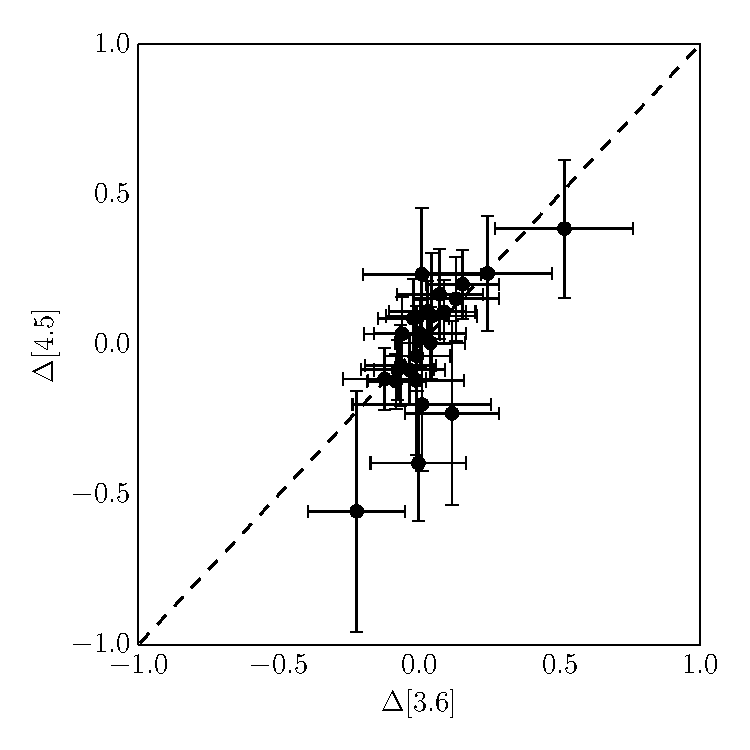
\includegraphics[width=80mm]{reworked_fitting_code/final_plots/deltadelta_3p6_4p5_spect.pdf}
\caption{$\Delta$3.6~$\mu$m vs. $\Delta$4.5~$\mu$m using spectroscopic metallicities}
\label{fig:deltadelta_spect}
\end{center}
\end{figure}

\begin{figure}
\begin{center}
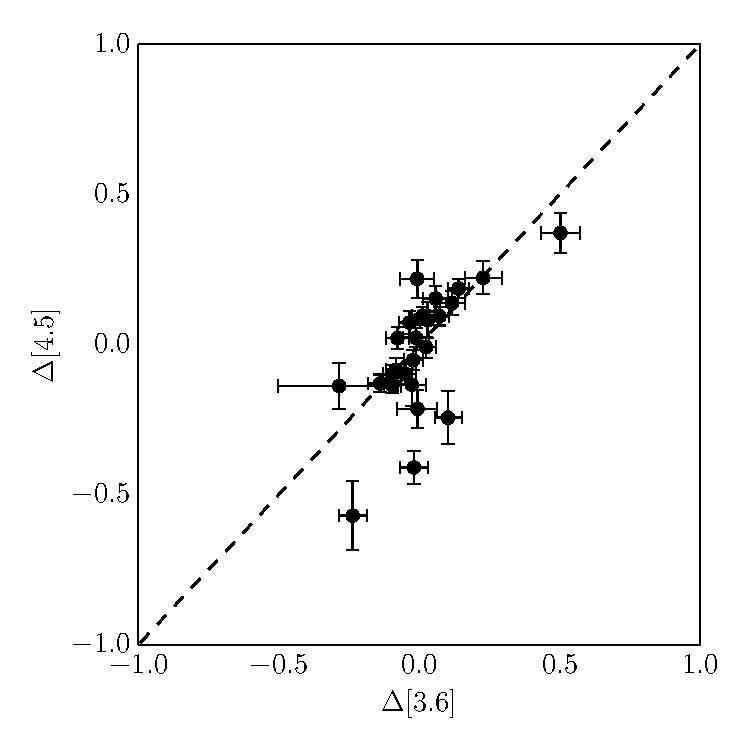
\includegraphics[width=80mm]{reworked_fitting_code/final_plots/deltadelta_3p6_4p5_phot.pdf}
\caption{$\Delta$3.6~$\mu$m vs. $\Delta$4.5~$\mu$m using photometric metallicities}
\label{fig:deltadelta_phot}
\end{center}
\end{figure}
\end{comment}


%%%%%%%%%%%%%%%%%%%%%%%%%%%%%%%%%%%%%%%%%%%%%%%%%%


% Don't change these lines
\bsp	% typesetting comment
\label{lastpage}
\end{document}

% End of mnras_template.tex